\section{Experiments and Results}
\label{sec:experiments_results}

MOSAIC was evaluated in the same order in which the method is used. The starting point is the supervision imbalance in the cohort: multimodal imaging and structured clinical evidence were available at scale, but clinician-authored reports were incomplete and highly uneven across centres. We therefore first quantify the report-supervision bottleneck, then test whether QC-gated pseudo reports contain modality-grounded semantic information beyond class-label templates. We next ask whether section-aware RASA alignment organises multimodal representations and whether pseudo-report supervision is most useful when real reports are scarce. After these mechanism-level tests, we evaluate the full MOSAIC predictor, which augments the MOSAIC--RASA backbone with a train-only semantic retrieval bank and validation-calibrated logit fusion. Semantic-tag analysis, QC stress testing, perturbation, strict leave-one-centre-out evaluation, robustness checks, and scalability analyses are then used to delimit the strength of the retrospective evidence.

All analyses used the locked retrospective five-centre cohort and the fixed train/validation/test split of 1,325/284/288 cases. Test labels were used only for final metric computation and bootstrap resampling. Pseudo-report construction, retrieval-bank construction, fusion-weight selection, and operating-threshold selection followed the training and validation protocol described in Methods. A reviewer-audit pass confirmed that the same-split MOSAIC, MOSAIC--RASA, semantic-retrieval, MOSAIC-Tag, clinical-only, image-only, fusion, cross-attention, and contrastive baseline prediction files all covered the same 288 locked test case identifiers. Table~\ref{tab:experiment_logic_map} maps each result block to the MOSAIC component it tests. The main text includes the completed provider, ablation, perturbation, semantic-tag, cross-centre, masking, robustness, and scalability experiments in prose, while the corresponding S tables and supplemental figures are grouped in Supplementary Appendix~\ref{sec:supplementary_experiments_results}.

\begin{figure*}[!htbp]
  \centering
  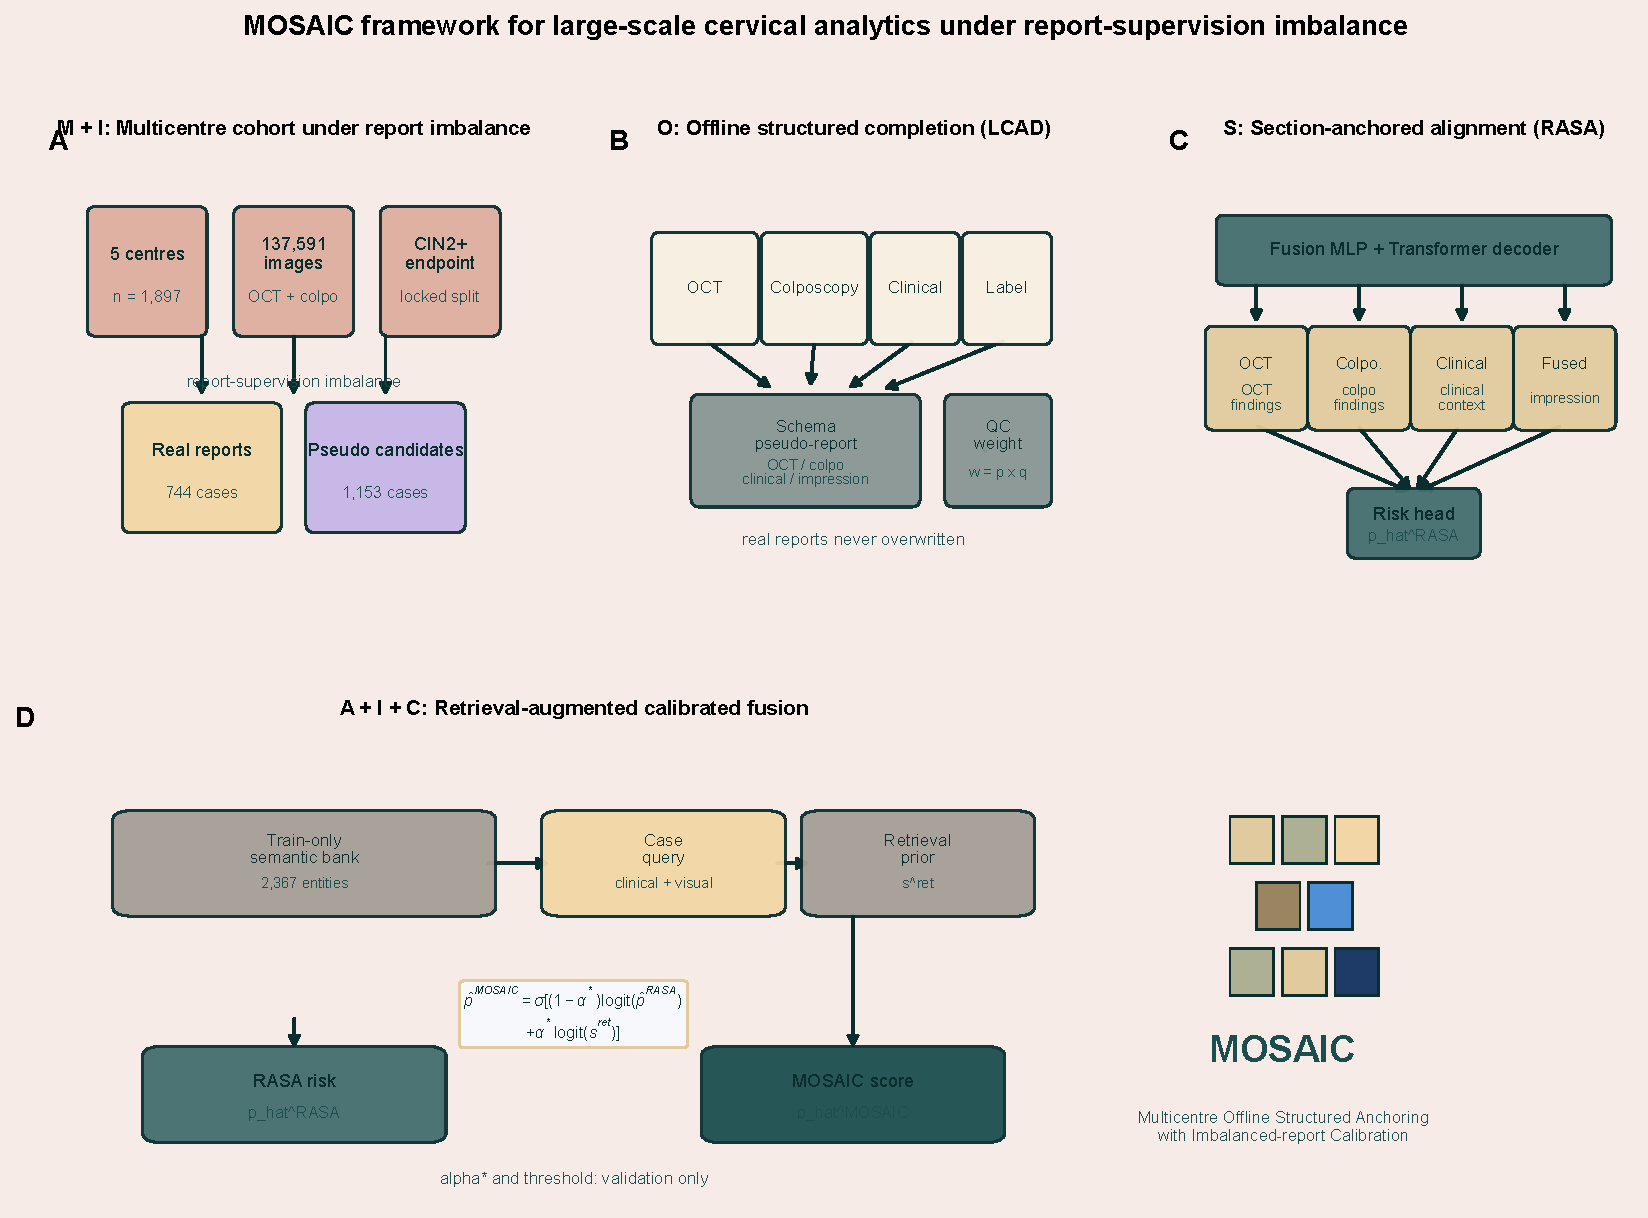
\includegraphics[width=\linewidth]{final_Fig/Figure1_mosaic_overview.pdf}
  \caption{Overview of the MOSAIC framework. The evidence chain starts from a five-centre multimodal cohort with incomplete report supervision, uses offline weak-oracle structured completion for report-missing cases, aligns modality representations to report sections through MOSAIC--RASA, builds a semantic retrieval bank from training cases only, and applies validation-calibrated fusion before a single locked test evaluation.}
  \label{fig:mosaic_overview}
\end{figure*}

\begin{table*}[!htbp]
  \centering
  \caption{How each result block maps to MOSAIC method components.}
  \label{tab:experiment_logic_map}
  \scriptsize
  \begin{threeparttable}
  \resizebox{\linewidth}{!}{%
  \begin{tabular}{p{3.0cm}p{4.2cm}p{4.4cm}p{4.4cm}}
    \toprule
    \textbf{Result block} & \textbf{Method component being tested} & \textbf{Primary question} & \textbf{Main evidence used in this section} \\
    \midrule
    Cohort and supervision imbalance & Study design and weak-oracle problem formulation & Is there a real report-supervision bottleneck rather than only an image-scale problem? & Five-centre case, image, report, and pseudo-report counts; centre-level report coverage \\
    Weak-oracle report construction & Phase O: LCAD QC-gated completion & Do pseudo reports add modality-grounded semantics beyond class-label templates? & Source comparison, modality support, duplication, masking validation, provider feasibility audit \\
    Section alignment and scarcity & Phase S: RASA section anchors & Do report sections organise multimodal representations and help when real reports are scarce? & Modality-section retrieval, scarcity curve, pseudo-report-augmented surrogate \\
    Held-out risk stratification & Phase A+I+C: train-only retrieval and calibrated fusion & Does the semantic prior improve the locked test predictor over the backbone? & MOSAIC-RASA, retrieval-only, and MOSAIC test metrics; paired bootstrap audit \\
    Boundary and robustness audits & Tag retrieval, QC stress testing, perturbation, CIN3+ safety, LOCO, robustness & Which parts of the retrospective evidence remain limited? & MOSAIC-Tag secondary audit, failure-enriched QC, proxy CIN3+ safety table, perturbation matrix, strict LOCO, embedding and duplicate-leakage audits, scalability and stability \\
    \bottomrule
  \end{tabular}%
  }
  \end{threeparttable}
\end{table*}

\FloatBarrier

\subsection{Five-centre cohort and report-supervision bottleneck}
\label{subsec:cohort_results}

We first characterised the data available for learning. The final analytic cohort contained 1,897 multimodal cervical screening cases from five centres, comprising 129,030 OCT files, 8,561 colposcopy-associated files, and 137,591 total evaluable image files (Table~\ref{tab:baseline_all3000_5cens}). Archived clinician-authored reports were available for 744 cases. The other 1,153 cases retained multimodal evidence but lacked report-level textual supervision. A complete-case report-learning strategy would therefore discard most report-missing cases, despite their usable imaging and clinical information.

\begin{table*}[!htbp]
  \centering
  \caption{Five-centre cohort scale and report-supervision availability.}
  \label{tab:baseline_all3000_5cens}
  \scriptsize
  \begin{threeparttable}
  \resizebox{\linewidth}{!}{%
  \begin{tabular}{lrrrrr}
    \toprule
    \textbf{Centre} & \textbf{Cases} & \textbf{OCT images} & \textbf{Colposcopy images} & \textbf{Real reports} & \textbf{Pseudo-report candidates} \\
    \midrule
    Enshi Central Hospital & 406 & 48,504 & 1,233 & 406 & 0 \\
    Jingzhou First People's Hospital & 406 & 12,428 & 2,967 & 334 & 72 \\
    Shiyan People's Hospital & 496 & 14,267 & 1,488 & 0 & 496 \\
    Renmin Hospital of Wuhan University & 89 & 10,680 & 267 & 0 & 89 \\
    Xiangyang Central Hospital & 500 & 43,151 & 2,606 & 4 & 496 \\
    \midrule
    \textbf{Overall} & \textbf{1,897} & \textbf{129,030} & \textbf{8,561} & \textbf{744} & \textbf{1,153} \\
    \bottomrule
  \end{tabular}%
  }
  \begin{tablenotes}[flushleft]
    \footnotesize
    \item Image counts were recomputed from the canonical case manifest. Archived-report status describes source-document availability only and was not used as a model input. The locked test set contained 288 cases.
  \end{tablenotes}
  \end{threeparttable}
\end{table*}

\begin{figure}[!htbp]
  \centering
  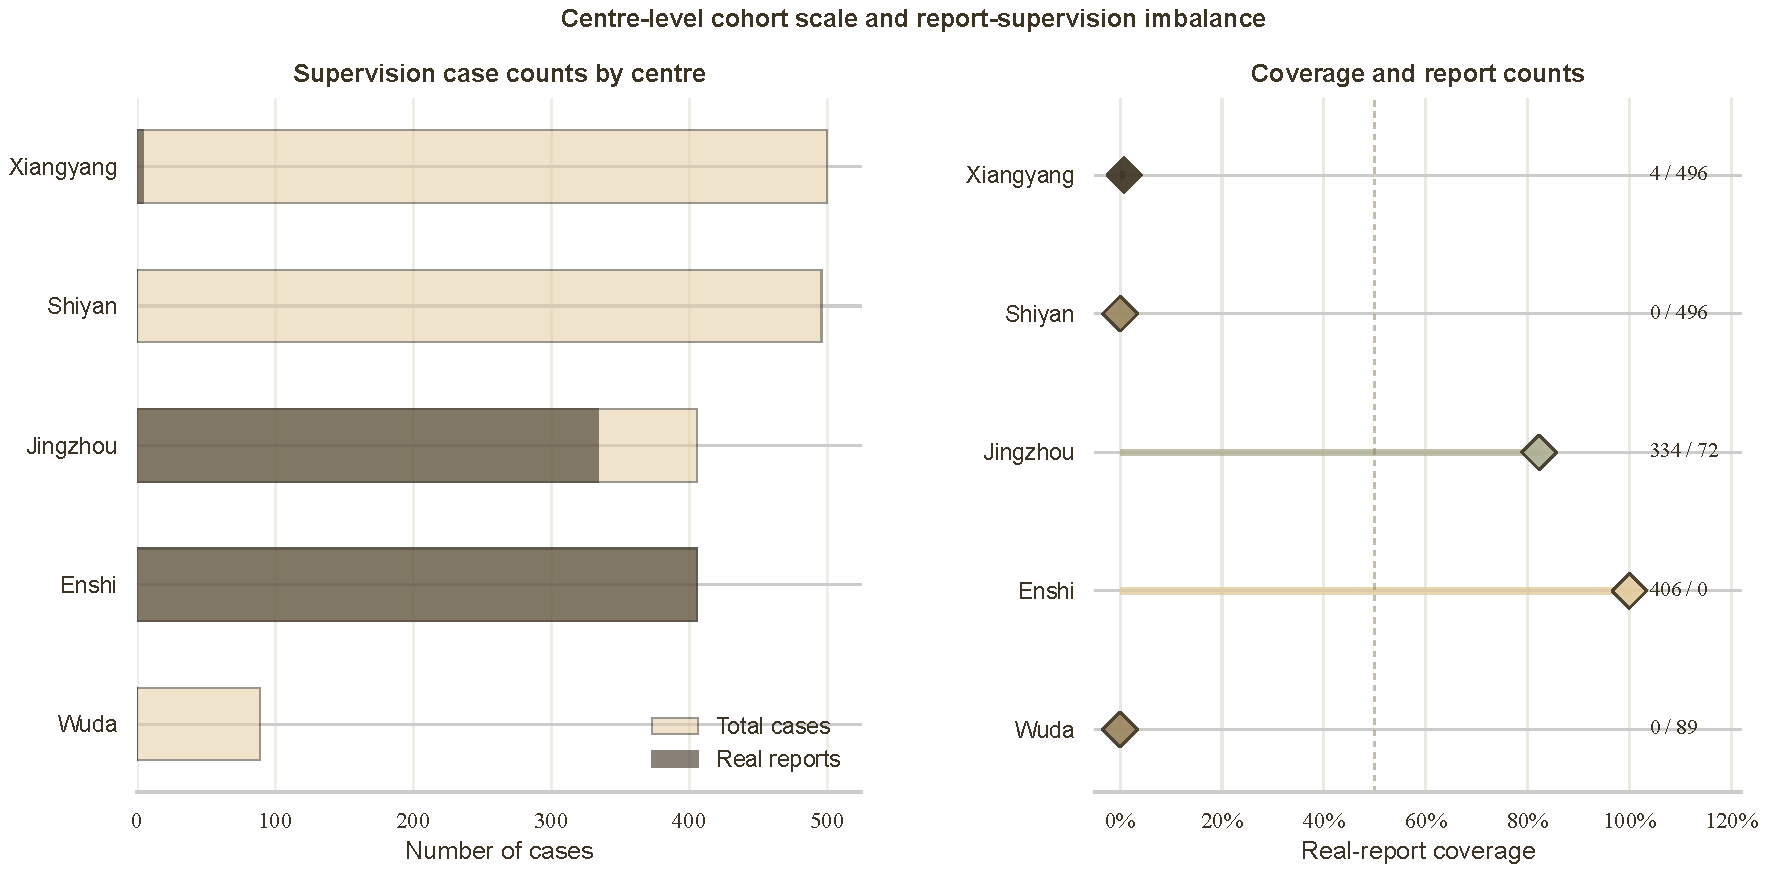
\includegraphics[width=\linewidth]{final_Fig/Figure2_centre_supervision_catplot.pdf}
  \caption{Centre-stratified report-supervision imbalance. Case counts and image volume were large across centres, but report coverage was highly uneven, motivating the weak-oracle formulation rather than a complete-case-only analysis.}
  \label{fig:centre_supervision}
\end{figure}

Report availability also varied by centre. Enshi retained reports for all 406 cases, Jingzhou for 334 of 406 cases, Xiangyang for only 4 of 500 cases, and Wuhan and Shiyan had no centre-wide report archive. This centre-dependent missingness is the supervision bottleneck addressed by MOSAIC. Generated text is therefore not treated as physician-authored documentation. It is used as QC-gated weak semantic supervision so that report-missing cases can still contribute structured targets, while archival reports and generated supervision remain clearly separated.

\FloatBarrier

\subsection{Weak-oracle pseudo reports carry more signal than label templates}
\label{subsec:pseudo_report_results}

The next question was whether pseudo reports added usable semantic structure or merely restated diagnostic labels. The label-template source served as a negative control. It produced schema-complete reports, but showed no modality support and had a high maximum duplicate fraction of 0.867 (Table~\ref{tab:pseudo_source_comparison}). Thus, schema completion alone was not enough for weak-oracle supervision: report-shaped text could still be repetitive and ungrounded.

\begin{table*}[!htbp]
  \centering
  \caption{Structured pseudo-report source comparison.}
  \label{tab:pseudo_source_comparison}
  \scriptsize
  \begin{threeparttable}
  \resizebox{\linewidth}{!}{%
  \begin{tabular}{lrrrrr}
    \toprule
    \textbf{Source} & \textbf{$n$} & \textbf{Label consistency} & \textbf{Modality support} & \textbf{Unique text} & \textbf{Duplicate fraction} \\
    \midrule
    Label template & 180 & 0.567 & 0.000 & 0.011 & 0.867 \\
    Rule-based & 180 & \textbf{0.628} & \textbf{1.000} & \textbf{0.194} & \textbf{0.200} \\
    Local embedding-assisted LLM & 180 & \textbf{0.628} & \textbf{1.000} & 0.156 & 0.261 \\
    \bottomrule
  \end{tabular}%
  }
  \begin{tablenotes}[flushleft]
    \footnotesize
    \item All sources produced schema-complete reports, so the complete-rate column was omitted. Pseudo reports are used as weighted semantic supervision, not as clinical ground truth.
  \end{tablenotes}
  \end{threeparttable}
\end{table*}

\begin{figure}[!htbp]
  \centering
  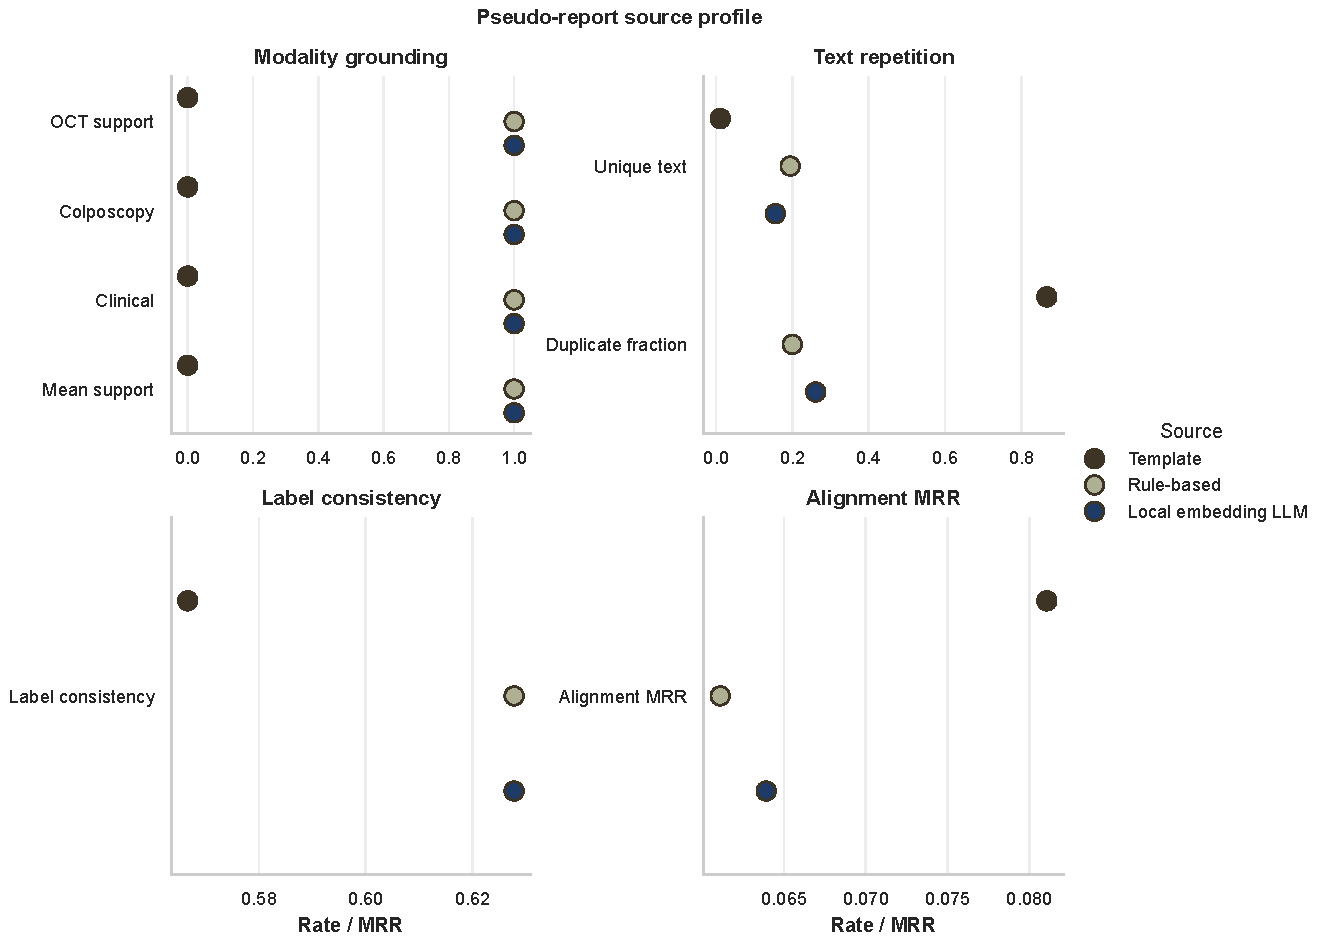
\includegraphics[width=\linewidth]{final_Fig/Figure_theme1_pseudo_report_source_comparison.pdf}
  \caption{Structured pseudo-report source comparison. The label-template control shows that schema completion alone can be repetitive and ungrounded, whereas rule-based and local embedding-assisted LLM reports preserve modality-specific support.}
  \label{fig:pseudo_source_comparison}
\end{figure}

The rule-based and local embedding-assisted LLM sources were more useful for this purpose. Both achieved modality-support rates of 1.000, higher label-consistency values, and substantially lower duplicate fractions than the label-template control. Phase O is therefore justified by evidence-grounded structured completion, not by text generation alone. In this study, a ``weak oracle'' means a quality-weighted semantic prior for representation learning whose sections remain tied to OCT findings, colposcopy findings, and clinical context. It is not a substitute for clinician-authored ground truth.

External provider analyses were used as implementation audits rather than as the default MOSAIC training source. Only de-identified structured evidence was transmitted; raw images, image paths, patient names, internal identifiers, hospital identifiers, and directly identifying information were not sent to external providers. In the extended 100-case API cohort, GPT-5.5 produced 100 schema-valid structured reports, with section completeness 0.810, modality support 0.810, contradiction rate 0.050, hallucination rate 0.000, mean latency 11.39 seconds per case, and estimated cost of US\$27.73 per 1,000 cases. The Qwen-Plus, GLM-4.7-Flash, and Gemini-3.1-Pro cohorts were smaller pilots, so they are reported as feasibility and operational-reliability checks rather than definitive provider rankings.

Two additional controls strengthened the Phase O interpretation. First, all 1,153 pseudo-report candidates passed the implemented structured-output QC screen in the clean retrospective run, supporting cohort-scale feasibility while not proving clinical validity. Second, masking validation compared label-only agents with modality-conditioned agents. On Enshi, the label-consistency proxy increased from 0.659 under label-only generation to 0.746 when modality evidence was available; in the pooled Enshi--Jingzhou subset, it increased from 0.593 to 0.664. These results indicate that generated sections were conditioned on multimodal evidence, although they remain proxy audits rather than expert physician ratings.

\FloatBarrier

\subsection{Section-aware alignment and scarcity analyses support the weak-oracle mechanism}
\label{subsec:alignment_scarcity_results}

After excluding a label-template explanation, we tested whether report sections helped organise the multimodal representation space. Phase S was evaluated with a modality-section retrieval audit: OCT embeddings queried \texttt{oct\_findings}, colposcopy embeddings queried \texttt{colposcopy\_findings}, clinical embeddings queried \texttt{clinical\_context}, and fused representations queried \texttt{impression}. The MOSAIC--RASA backbone achieved macro MRR 0.051, compared with 0.021 after removing section alignment and 0.022 under simple concatenation fusion (Table~\ref{tab:theme1_alignment_ablation}). The absolute retrieval values were modest, so this result should be read as evidence of relative section-wise organisation under a difficult audit, not as high-fidelity open-ended semantic retrieval.

\begin{table*}[!htbp]
  \centering
  \caption{Direct RASA alignment ablation using modality-section retrieval.}
  \label{tab:theme1_alignment_ablation}
  \scriptsize
  \begin{threeparttable}
  \resizebox{\linewidth}{!}{%
  \begin{tabular}{lrrrr}
    \toprule
    \textbf{Model} & \textbf{Recall@1} & \textbf{Recall@5} & \textbf{Macro MRR} & \textbf{Positive cosine} \\
    \midrule
    Real-report only & \textbf{0.0182} & 0.0642 & \textbf{0.057} & \textbf{0.984} \\
    Pseudo-augmented LCAD & 0.0139 & \textbf{0.0729} & 0.055 & \textbf{0.984} \\
    MOSAIC--RASA backbone & 0.0148 & 0.0608 & 0.051 & \textbf{0.984} \\
    No section alignment & 0.0052 & 0.0139 & 0.021 & 0.013 \\
    Simple concatenation fusion & 0.0035 & 0.0182 & 0.022 & 0.021 \\
    \bottomrule
  \end{tabular}%
  }
  \end{threeparttable}
\end{table*}

\begin{figure*}[!htbp]
  \centering
  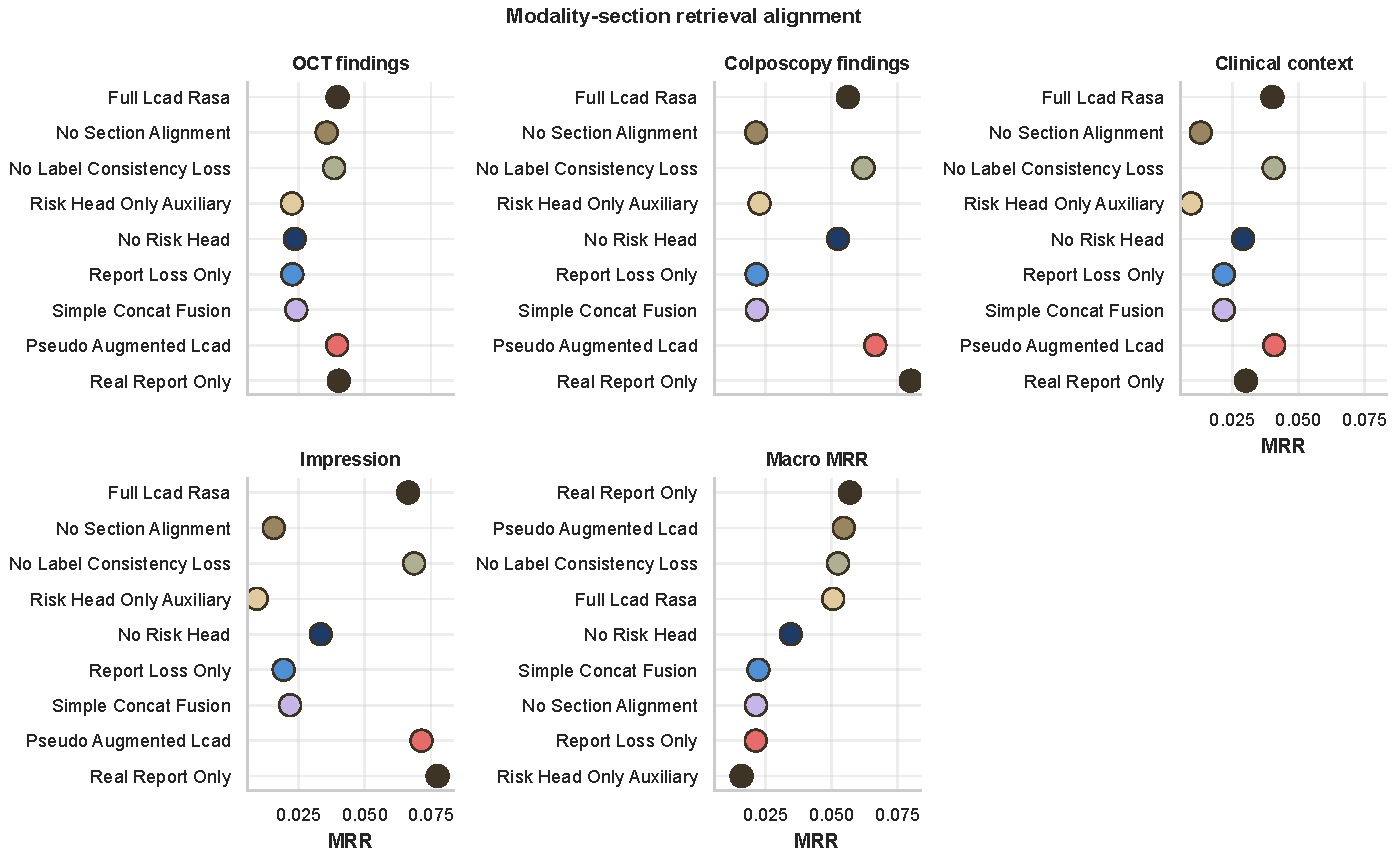
\includegraphics[width=0.49\linewidth]{final_Fig/Figure_theme1_alignment_retrieval_mrr.pdf}
  \hfill
  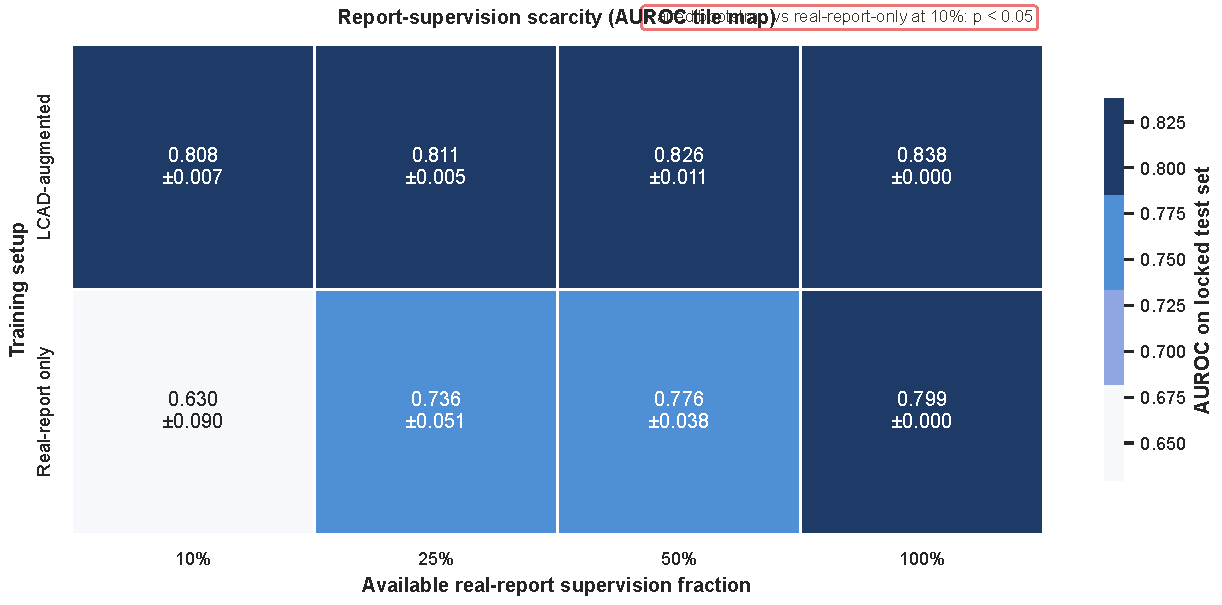
\includegraphics[width=0.49\linewidth]{final_Fig/Figure_theme1_report_supervision_scarcity_curve.pdf}
  \caption{Mechanism analyses for section-aware weak supervision. Left: modality-section retrieval tests whether RASA aligns each modality with its corresponding report section. Right: the report-scarcity curve tests whether pseudo-report augmentation is most useful when real report supervision is limited.}
  \label{fig:alignment_and_scarcity}
\end{figure*}

The scarcity experiment then asked whether the alignment signal mattered most when real reports were limited. With only 10\% of real-report supervision retained, the LCAD-augmented surrogate achieved AUROC 0.808 and F1 0.500, compared with AUROC 0.630 and F1 0.316 for the real-report-only surrogate (Table~\ref{tab:scarcity_curve}). The gap narrowed when full real-report supervision was available, but it did not disappear. This pattern matches the intended use of MOSAIC: pseudo-report supervision is most valuable when image and clinical evidence are abundant but report-level semantic supervision is scarce.

Provider-specific alignment and scarcity analyses checked whether the structured-report layer could be implemented with different generators. In the staged API audit, Gemini-3.1-Pro had the strongest pilot macro MRR among the available provider cohorts, whereas GPT-5.5 provided the larger 100-case operational cohort and the most favourable low-contradiction, low-latency profile. In downstream scarcity surrogates using API-generated pseudo reports, GPT-5.5 at 10\% real-report availability achieved AUROC 0.630 and F1 0.229, while Gemini-3.1-Pro achieved AUROC 0.725 and F1 0.379 in its smaller valid pilot cohort. These experiments remain provider feasibility and operational sensitivity analyses; they are not substitutes for full MOSAIC retraining.

\begin{table*}[!htbp]
  \centering
  \caption{Report-supervision scarcity curve using a lightweight downstream surrogate.}
  \label{tab:scarcity_curve}
  \scriptsize
  \begin{threeparttable}
  \resizebox{\linewidth}{!}{%
  \begin{tabular}{llrrrrr}
    \toprule
    \textbf{Real-report fraction} & \textbf{Setup} & \textbf{Train $n$} & \textbf{Real $n$} & \textbf{Pseudo $n$} & \textbf{AUROC} & \textbf{F1} \\
    \midrule
    1.00 & LCAD-augmented surrogate & 1,325 & 520 & 805 & \textbf{0.838} & \textbf{0.542} \\
    1.00 & Real-report-only surrogate & 520 & 520 & 0 & 0.799 & 0.471 \\
    0.50 & LCAD-augmented surrogate & 1,065 & 260 & 805 & \textbf{0.826} & \textbf{0.526} \\
    0.50 & Real-report-only surrogate & 260 & 260 & 0 & 0.776 & 0.442 \\
    0.25 & LCAD-augmented surrogate & 935 & 130 & 805 & \textbf{0.811} & \textbf{0.485} \\
    0.25 & Real-report-only surrogate & 130 & 130 & 0 & 0.736 & 0.383 \\
    0.10 & LCAD-augmented surrogate & 857 & 52 & 805 & \textbf{0.808} & \textbf{0.500} \\
    0.10 & Real-report-only surrogate & 52 & 52 & 0 & 0.630 & 0.316 \\
    \bottomrule
  \end{tabular}%
  }
  \end{threeparttable}
\end{table*}

\FloatBarrier

\subsection{Train-only semantic retrieval improves locked held-out risk stratification}
\label{subsec:mosaic_main_results}

The mechanism analyses support the use of weak-oracle semantic supervision. We next tested whether that structure improved risk prediction under the locked evaluation protocol. The full MOSAIC predictor adds Phase A+I+C semantic priors to the MOSAIC--RASA backbone. The retrieval bank contained training-derived cervical section entities only; validation and test labels were excluded from bank construction. On the locked held-out test set (\(n=288\)), the MOSAIC--RASA backbone achieved AUROC 0.856, AUPRC 0.662, and F1 0.519 (Table~\ref{tab:mosaic_main}). Semantic retrieval alone was informative but insufficient as a standalone predictor, with AUROC 0.774 and F1 0.585. After validation-calibrated logit fusion (\(\alpha=0.31\)) and a validation-selected threshold of 0.50, MOSAIC achieved AUROC 0.908, AUPRC 0.741, F1 0.736, sensitivity 0.727, precision 0.744, and balanced accuracy 0.841.

\begin{table*}[!htbp]
  \centering
  \caption{Locked held-out test performance of the MOSAIC semantic-prior pipeline.}
  \label{tab:mosaic_main}
  \scriptsize
  \begin{threeparttable}
  \resizebox{\linewidth}{!}{%
  \begin{tabular}{lrrrrrrr}
    \toprule
    \textbf{Method} & \textbf{AUROC} & \textbf{AUPRC} & \textbf{F1} & \textbf{Sensitivity} & \textbf{Precision} & \textbf{Balanced accuracy} & \textbf{Threshold} \\
    \midrule
    MOSAIC--RASA backbone & 0.856 & 0.662 & 0.519 & 0.636 & 0.438 & 0.744 & 0.39 \\
    Semantic retrieval only & 0.774 & 0.589 & 0.585 & 0.545 & 0.632 & 0.744 & 0.67 \\
    \textbf{MOSAIC} & \textbf{0.908} & \textbf{0.741} & \textbf{0.736} & \textbf{0.727} & \textbf{0.744} & \textbf{0.841} & 0.50 \\
    \bottomrule
  \end{tabular}%
  }
  \begin{tablenotes}[flushleft]
    \footnotesize
    \item The semantic retrieval bank was built from the training split only. The fusion weight and threshold were selected on the validation split and locked before test evaluation.
  \end{tablenotes}
  \end{threeparttable}
\end{table*}

\begin{figure}[!htbp]
  \centering
  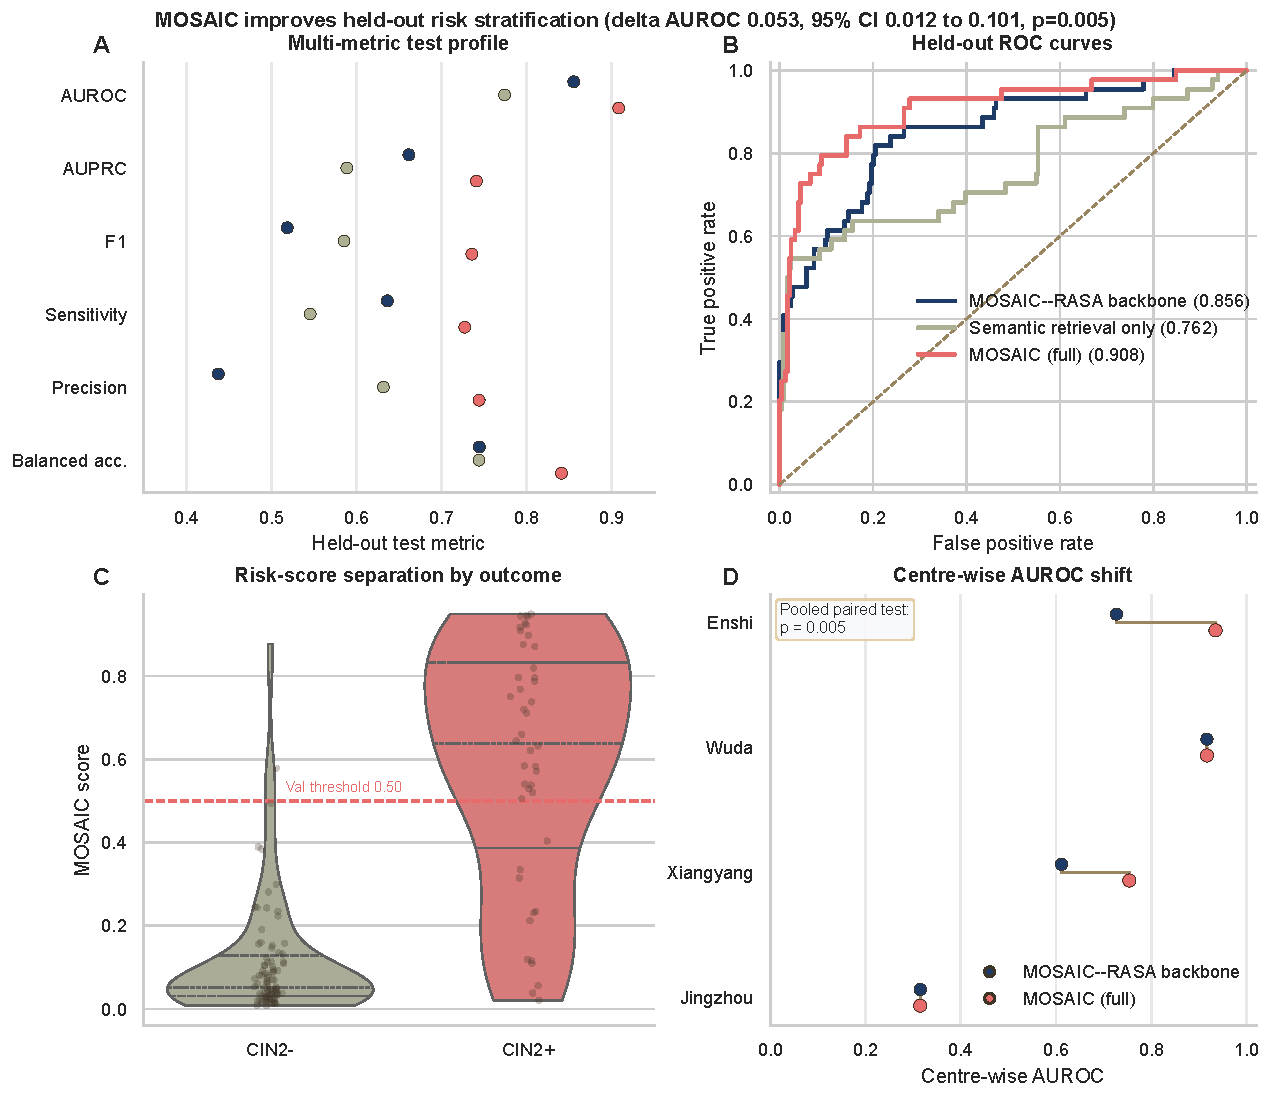
\includegraphics[width=\linewidth]{final_Fig/Figure_mosaic_performance_summary.pdf}
  \caption{Primary MOSAIC held-out performance. The figure summarises the backbone, retrieval-only prior, and fused MOSAIC predictor, including discrimination, score separation, and centre-wise AUROC shifts.}
  \label{fig:mosaic_performance_summary}
\end{figure}

The paired bootstrap audit showed incremental value beyond the backbone. MOSAIC improved AUROC by 0.053 over MOSAIC--RASA (95\% CI, 0.012--0.101; two-sided \(p=0.005\); 2,000 resamples). This is the primary predictive result in the section. Its interpretation is deliberately narrow: under the locked retrospective protocol, train-only semantic memory contributed risk information beyond the RASA backbone. Prospective clinical utility still requires prospective validation.

For continuity with the earlier LCAD--RASA experiment stack, we retained the pre-retrieval protocol-harmonisation analysis. In that analysis, the full pre-retrieval MOSAIC--RASA block reached AUROC 0.832 [0.757, 0.897] and F1 0.611 [0.458, 0.737] at threshold 0.37; pseudo-augmented LCAD reached AUROC 0.826 [0.747, 0.894] and F1 0.545 at threshold 0.39; real-report-only training reached AUROC 0.725; and simple concatenation remained substantially lower. These historical backbone comparisons explain why the section-aware architecture was retained, while the primary manuscript result is the later full MOSAIC model with train-only semantic retrieval and validation-calibrated fusion.

\FloatBarrier

\subsection{Same-split baseline comparison calibrates the strength of the claim}
\label{subsec:external_baseline_results}

We then placed MOSAIC against same-split clinical-only, image-only, late-fusion, cross-attention, and contrastive multimodal baselines. MOSAIC had the highest AUROC point estimate (0.908; 95\% CI, 0.845--0.957), followed by the CLIP-style contrastive multimodal baseline (0.888; 95\% CI, 0.821--0.942) and clinical-only HistGradientBoosting (0.862; 95\% CI, 0.798--0.918) (Table~\ref{tab:external_baselines}). The comparison also clarifies the contribution. The MOSAIC--RASA backbone alone did not dominate the strongest contrastive baseline. The empirical gain therefore lies in the complete weak-oracle semantic-prior pipeline with train-only retrieval and validation-calibrated fusion, not in the backbone alone.

\begin{table*}[!htbp]
  \centering
  \caption{Same-split comparison with external baselines on the locked held-out test set.}
  \label{tab:external_baselines}
  \scriptsize
  \begin{threeparttable}
  \resizebox{\linewidth}{!}{%
  \begin{tabular}{lrrr}
    \toprule
    \textbf{Model} & \textbf{AUROC [95\% CI]} & \textbf{F1 [95\% CI]} & \textbf{Threshold} \\
    \midrule
    \textbf{MOSAIC} & \textbf{0.908 [0.845, 0.957]} & \textbf{0.736 [0.620, 0.830]} & 0.50 \\
    CLIP-style contrastive multimodal baseline & 0.888 [0.821, 0.942] & 0.640 [0.500, 0.753] & 0.79 \\
    Clinical-only HistGradientBoosting & 0.862 [0.798, 0.918] & 0.632 [0.507, 0.741] & 0.68 \\
    MOSAIC--RASA backbone & 0.856 [0.782, 0.915] & 0.519 [0.411, 0.667] & 0.39 \\
    Cross-attention multimodal transformer & 0.847 [0.776, 0.908] & 0.522 [0.385, 0.636] & 0.65 \\
    Clinical-only logistic regression & 0.830 [0.760, 0.889] & 0.557 [0.430, 0.673] & 0.63 \\
    Colposcopy-only embedding MLP & 0.827 [0.756, 0.890] & 0.510 [0.381, 0.627] & 0.74 \\
    Late-fusion MLP & 0.824 [0.750, 0.891] & 0.486 [0.333, 0.625] & 0.77 \\
    OCT-only embedding MLP & 0.786 [0.708, 0.861] & 0.494 [0.344, 0.622] & 0.68 \\
    \bottomrule
  \end{tabular}%
  }
  \begin{tablenotes}[flushleft]
    \footnotesize
    \item All rows used the same train/validation/test split, validation-selected threshold rule, held-out test set, and bootstrap confidence-interval protocol.
  \end{tablenotes}
  \end{threeparttable}
\end{table*}

\begin{figure}[!htbp]
  \centering
  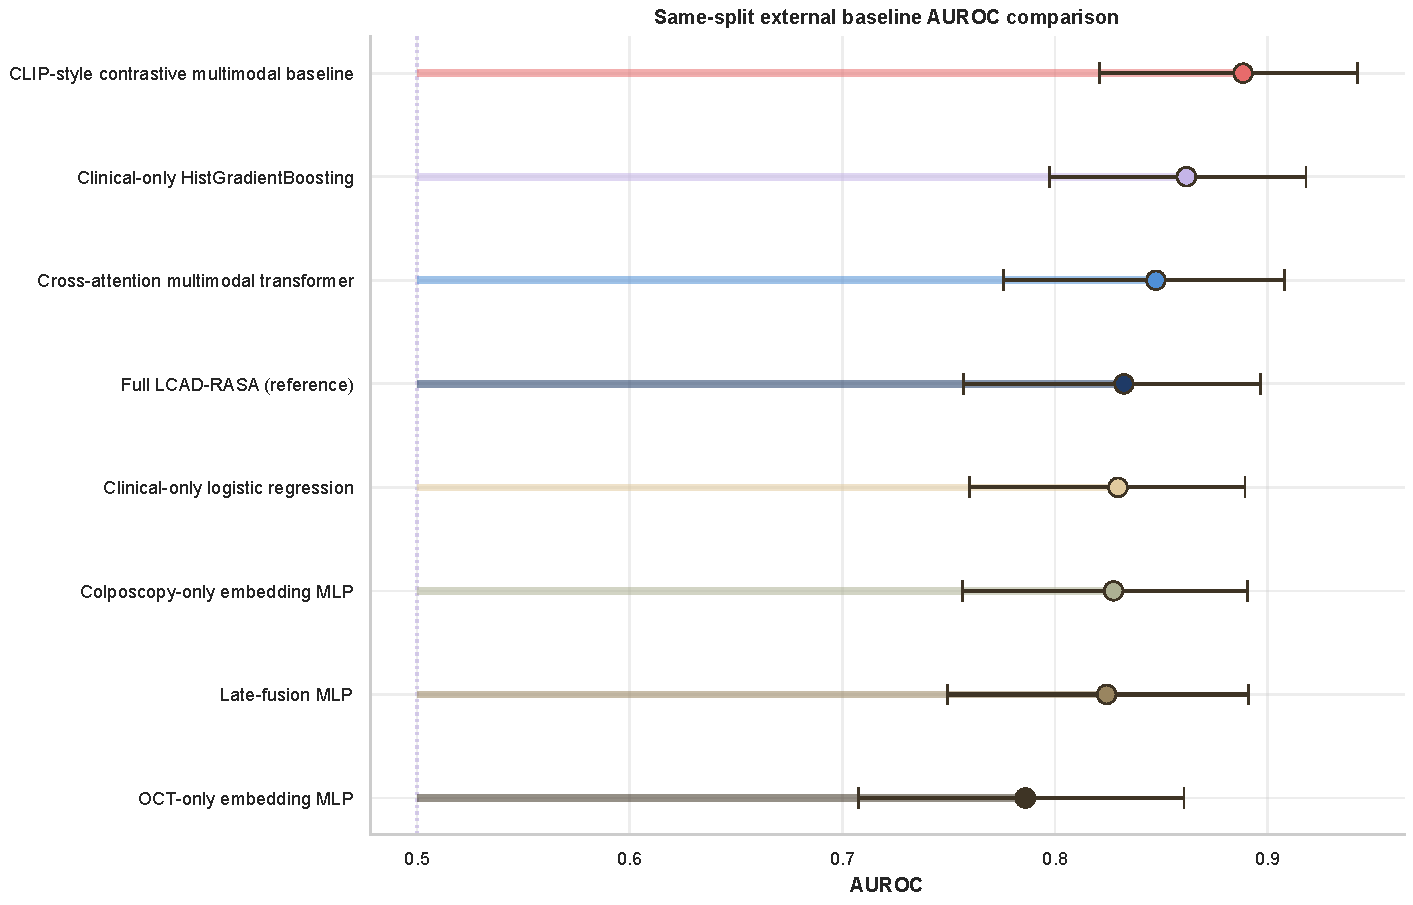
\includegraphics[width=\linewidth]{final_Fig/Figure_external_baselines_auc_forest.pdf}
  \caption{Same-split AUROC comparison against external baselines. Intervals denote bootstrap 95\% confidence intervals on the locked held-out test set.}
  \label{fig:external_baselines_auc}
\end{figure}

The paired comparisons refine this interpretation (Table~\ref{tab:full_mosaic_paired_bootstrap}). MOSAIC exceeded the CLIP-style contrastive baseline by point estimate, but the paired AUROC interval crossed zero (\(\Delta\)AUROC 0.020; 95\% CI, -0.019--0.065; \(p=0.355\)). The result therefore does not support a broad claim that MOSAIC is superior to every strong multimodal baseline. It supports a narrower claim: incomplete report supervision can be converted into leakage-controlled semantic priors that significantly improve MOSAIC over its own backbone and remain competitive with strong same-split multimodal alternatives.

The extended external-baseline profile also included metric dot plots and paired-delta rechecks. These analyses are important because the backbone itself did not uniformly dominate non-report baselines: the CLIP-style contrastive model exceeded the MOSAIC--RASA backbone before semantic retrieval, and clinical-only HistGradientBoosting remained a strong same-split comparator. This pattern frames MOSAIC as a report-supervision and semantic-prior framework rather than as a generic assertion that every report-aware component outperforms every discriminative multimodal baseline.

\begin{table*}[!htbp]
  \centering
  \caption{Paired-bootstrap comparison of MOSAIC with same-split comparators. Positive deltas favour MOSAIC.}
  \label{tab:full_mosaic_paired_bootstrap}
  \scriptsize
  \begin{threeparttable}
  \resizebox{\linewidth}{!}{%
  \begin{tabular}{lrrrr}
    \toprule
    \textbf{Comparator} & \textbf{Comparator AUROC} & \textbf{\(\Delta\)AUROC} & \textbf{95\% interval} & \textbf{Two-sided \(p\)} \\
    \midrule
    CLIP-style contrastive multimodal baseline & 0.888 & 0.020 & [-0.019, 0.065] & 0.355 \\
    Clinical-only HistGradientBoosting & 0.862 & 0.047 & [-0.015, 0.111] & 0.151 \\
    MOSAIC--RASA backbone & 0.856 & 0.053 & [0.012, 0.101] & \textbf{0.005} \\
    Cross-attention multimodal transformer & 0.847 & 0.061 & [0.013, 0.113] & \textbf{0.011} \\
    Clinical-only logistic regression & 0.830 & 0.079 & [0.026, 0.136] & \textbf{0.003} \\
    Colposcopy-only embedding MLP & 0.827 & 0.081 & [0.028, 0.142] & \textbf{0.002} \\
    Late-fusion MLP & 0.824 & 0.084 & [0.028, 0.145] & \textbf{0.002} \\
    OCT-only embedding MLP & 0.786 & 0.122 & [0.052, 0.197] & \textbf{\(<0.001\)} \\
    \bottomrule
  \end{tabular}%
  }
  \begin{tablenotes}[flushleft]
    \footnotesize
    \item Comparisons used case-aligned held-out test predictions and 2,000 paired bootstrap resamples. Statistically supported rows are highlighted only to describe uncertainty under this protocol, not to claim clinical superiority.
  \end{tablenotes}
  \end{threeparttable}
\end{table*}

\FloatBarrier

\subsection{CIN3+ proxy safety-oriented threshold analysis}
\label{subsec:cin3_safety_results}

Because cervical-screening triage must consider high-grade disease safety, we added a CIN3+ safety audit using a conservative pathology-text proxy. The proxy counted explicit CIN3/CIN 3, AIS or carcinoma wording as CIN3+ and did not treat generic high-grade language alone as CIN3+. It is therefore used as a retrospective safety audit rather than as a locked clinically curated CIN3+ endpoint. Under the validation-selected CIN2+ F1 threshold, MOSAIC detected 17 of 20 proxy CIN3+ cases in the locked test set, with proxy CIN3+ sensitivity 0.850, specificity 0.903, NPV 0.988, and three false negatives (Table~\ref{tab:cin3_proxy_safety}). At the validation-selected high-sensitivity operating point targeting proxy CIN3+ sensitivity \(\geq 0.95\), MOSAIC detected 19 of 20 proxy CIN3+ cases, reducing false negatives to one while increasing positive calls from 43 to 66 and lowering specificity to 0.825.

\begin{table*}[!htbp]
  \centering
  \caption{CIN3+ proxy safety-oriented threshold audit on the locked test set.}
  \label{tab:cin3_proxy_safety}
  \scriptsize
  \begin{threeparttable}
  \resizebox{\linewidth}{!}{%
  \begin{tabular}{llrrrrrr}
    \toprule
    \textbf{Model} & \textbf{Operating point} & \textbf{AUROC} & \textbf{Sensitivity} & \textbf{Specificity} & \textbf{NPV} & \textbf{FN} & \textbf{Positive calls} \\
    \midrule
    MOSAIC & CIN2+ validation-F1 threshold & \textbf{0.954} & 0.850 & 0.903 & 0.988 & 3 & 43 \\
    MOSAIC & proxy CIN3+ high-sensitivity threshold & \textbf{0.954} & \textbf{0.950} & 0.825 & \textbf{0.995} & \textbf{1} & 66 \\
    MOSAIC--RASA backbone & CIN2+ validation-F1 threshold & 0.890 & 0.800 & 0.821 & 0.982 & 4 & 64 \\
    CLIP-style contrastive baseline & CIN2+ validation-F1 threshold & 0.937 & 0.700 & \textbf{0.937} & 0.977 & 6 & 31 \\
    Clinical-only HistGradientBoosting & CIN2+ validation-F1 threshold & 0.859 & 0.700 & 0.862 & 0.975 & 6 & 51 \\
    Clinical-only logistic regression & CIN2+ validation-F1 threshold & 0.869 & 0.650 & 0.851 & 0.970 & 7 & 53 \\
    \bottomrule
  \end{tabular}%
  }
  \begin{tablenotes}[flushleft]
    \footnotesize
    \item The locked test set contained 20 proxy CIN3+ cases under the conservative pathology-text rule. The high-sensitivity threshold was selected on the validation split for MOSAIC only; external baseline validation predictions were not available in the current audit, so no test-tuned high-sensitivity threshold is reported for those rows.
  \end{tablenotes}
  \end{threeparttable}
\end{table*}

These safety-oriented results support retrospective risk stratification, not autonomous clinical deployment. The proxy endpoint should be replaced by a prospectively locked and clinically curated CIN3+ endpoint before any deployment or triage claim is made.

\FloatBarrier

\subsection{Semantic-tag and quality-control audits limit over-interpretation}
\label{subsec:semantic_tag_qc_results}

The semantic-tag audit tested whether a simpler tag-normalisation layer could reproduce part of the retrieval-calibrated signal. The initial uncleaned semantic-tag stream was excluded because it contained target- or identifier-like metadata fields. After strict redaction, the cleaned tag input covered all 1,897 cases and passed leakage screening in the training, validation, and test splits, with zero forbidden target-derived terms, path-like tokens, or identifier hits. No LLM API key or local LLM endpoint was configured for semantic tagging in the current execution, so direct LLM-tag rows are unavailable. The deterministic rule-tag fallback is reported as MOSAIC-Tag, a secondary audit rather than a replacement for the primary MOSAIC pipeline.

\begin{table*}[!htbp]
  \centering
  \caption{Semantic-tag audit and model-role boundary.}
  \label{tab:semantic_tag_role_boundary}
  \scriptsize
  \begin{threeparttable}
  \resizebox{\linewidth}{!}{%
  \begin{tabular}{lrrrrrp{4.2cm}}
    \toprule
    \textbf{Model or audit} & \textbf{AUROC} & \textbf{AUPRC} & \textbf{F1} & \textbf{Sensitivity} & \textbf{Specificity} & \textbf{Role in manuscript} \\
    \midrule
    MOSAIC & 0.908 & 0.741 & 0.736 & 0.727 & 0.955 & Primary full framework \\
    CLIP-style contrastive baseline & 0.888 & 0.739 & 0.640 & 0.545 & 0.971 & Strong same-split comparator \\
    MOSAIC-Tag & 0.878 & 0.695 & 0.556 & 0.568 & 0.914 & Secondary cleaned tag-retrieval audit \\
    MOSAIC--RASA backbone & 0.856 & 0.662 & 0.519 & 0.636 & 0.852 & Backbone before retrieval-calibrated semantic fusion \\
    Direct LLM-tag retrieval & N/A & N/A & N/A & N/A & N/A & Unavailable in current run; excluded from claims \\
    \bottomrule
  \end{tabular}%
  }
  \begin{tablenotes}[flushleft]
    \footnotesize
    \item MOSAIC-Tag improved over MOSAIC--RASA in AUROC (paired \(\Delta\)AUROC 0.023; 95\% CI, 0.003--0.042; \(p=0.020\)) but remained below MOSAIC and did not establish LLM-tag superiority.
  \end{tablenotes}
  \end{threeparttable}
\end{table*}

Quality control was interpreted in the same restrained way. Its role is to filter and weight weak supervision, not to act as a standalone AUROC-improvement mechanism. Because retrospective QC variants did not materially change downstream discrimination, we used a failure-enriched stress test to examine whether the verifier reacted to severe pseudo-report defects. The stress test corrupted pseudo reports with label--impression contradictions, unsupported high-grade terminology, modality swaps, missing sections, hallucinated modality findings, duplicate templates, and inconsistent recommendations. The QC and rule-verifier audit rejected, down-weighted, or flagged most corrupted reports, while the modality-swap corruption was not captured by the current rule-only detector (Table~\ref{tab:qc_failure_stress_test}). No LLM verifier comparison is claimed.

The ablation suite gives the same message at the component level. The RASA alignment-weight sweep peaked around a moderate \(\lambda_{\mathrm{align}}\) value, consistent with section alignment acting as a regulariser rather than as the sole driver of performance. Modality ablations showed that colposcopy and clinical instruction carried strong risk information, but no single channel justified the full semantic-prior claim by itself. RASA component ablations showed that section alignment, risk supervision, and label-consistency terms affected different operating metrics, while QC variants were nearly flat in downstream AUROC in the clean retrospective run. The failure-enriched QC audit is therefore the relevant evidence for report-safety filtering, whereas the discrimination claim rests on MOSAIC's held-out predictive comparison.

\begin{table}[!htbp]
  \centering
  \caption{Failure-enriched QC stress-test audit.}
  \label{tab:qc_failure_stress_test}
  \small
  \begin{threeparttable}
  \begin{tabular}{lrl}
    \toprule
    \textbf{Stress-test metric} & \textbf{Value} & \textbf{Interpretation} \\
    \midrule
    Clean pseudo-report QC pass rate & 1.000 & Clean baseline retained \\
    Corrupted pseudo-report QC pass rate & 0.716 & Corrupted variants partly rejected \\
    Mean QC score, clean vs corrupted & 1.000 vs 0.841 & Corrupted reports down-weighted \\
    Severe-error flag rate, clean vs corrupted & 0.000 vs 0.284 & Severe failures enriched among corrupted reports \\
    Contradiction detection rate & 1.000 & Expected contradiction flags detected \\
    Hallucination detection rate & 0.999 & Unsupported terminology detected \\
    Missing-section detection rate & 1.000 & Empty required sections detected \\
    Modality-swap detection rate & 0.000 & Residual detector limitation \\
    Duplicate-template detection rate & 1.000 & Repeated template text detected \\
    \bottomrule
  \end{tabular}
  \begin{tablenotes}[flushleft]
    \footnotesize
    \item The stress test used all 1,153 pseudo-report candidates and the current QC function. No retraining under corrupted reports was performed.
  \end{tablenotes}
  \end{threeparttable}
\end{table}

\FloatBarrier

\subsection{Perturbation audits show modality-grounded decoding without implying causality}
\label{subsec:perturbation_results}

Perturbation analysis checked whether generated report sections changed when their corresponding input modalities were disrupted. The expected section-specific pattern was observed (Table~\ref{tab:perturbation_matrix}). Masking OCT produced a 0.743 drop in the OCT findings section, masking colposcopy produced a 1.000 drop in the colposcopy findings section, and masking clinical instruction produced a 0.833 drop in the clinical-context section. These matched degradations are consistent with modality-sensitive decoding rather than fixed-template completion.

\begin{table*}[!htbp]
  \centering
  \caption{Perturbation sensitivity matrix. Drops are relative to normal decoding.}
  \label{tab:perturbation_matrix}
  \scriptsize
  \begin{threeparttable}
  \resizebox{\linewidth}{!}{%
  \begin{tabular}{lrrrrr}
    \toprule
    \textbf{Condition} & \textbf{OCT drop} & \textbf{Colposcopy drop} & \textbf{Clinical drop} & \textbf{Report drop} & \textbf{\(|\Delta\)risk|} \\
    \midrule
    Mask OCT & 0.743 & 0.000 & 0.000 & 0.211 & 0.053 \\
    Shuffle OCT & 0.839 & 0.000 & 0.000 & 0.196 & 0.020 \\
    Mask colposcopy & 0.000 & \textbf{1.000} & 0.000 & 0.177 & 0.148 \\
    Shuffle colposcopy & 0.000 & 0.999 & 0.000 & 0.131 & 0.008 \\
    Mask instruction & 0.000 & 0.000 & 0.833 & 0.179 & 0.027 \\
    Shuffle instruction & 0.000 & 0.000 & 0.917 & 0.141 & 0.000 \\
    Mask visual evidence & 0.743 & \textbf{1.000} & 0.000 & 0.320 & 0.313 \\
    Label-only inference & 0.743 & \textbf{1.000} & 0.833 & \textbf{0.466} & \textbf{0.371} \\
    \bottomrule
  \end{tabular}%
  }
  \begin{tablenotes}[flushleft]
    \footnotesize
    \item Perturbation results are behavioural audits of modality sensitivity. They do not establish causal clinical reasoning or prospective interpretability.
  \end{tablenotes}
  \end{threeparttable}
\end{table*}

\begin{figure}[!htbp]
  \centering
  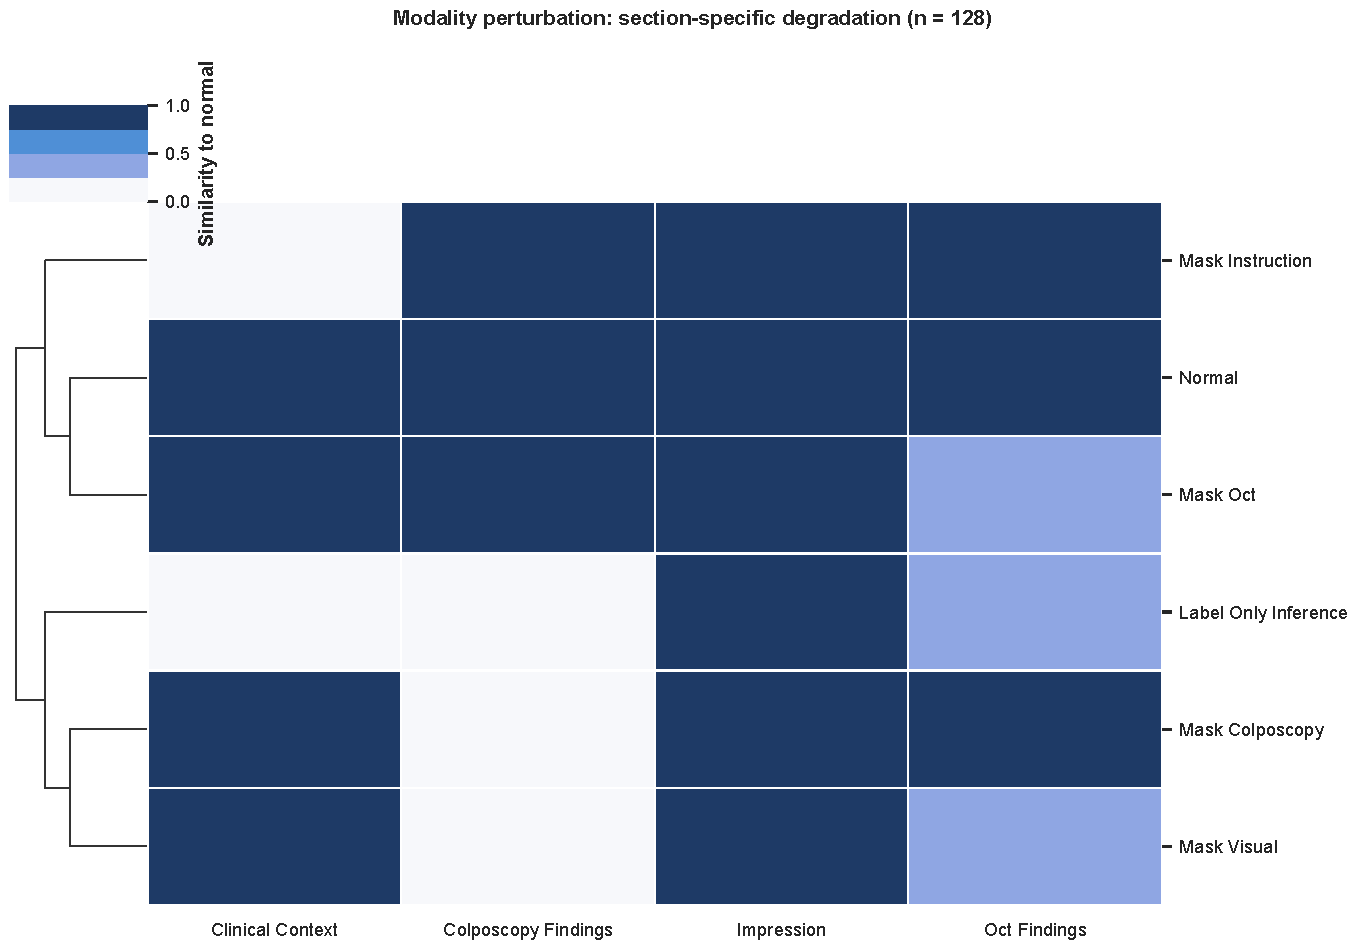
\includegraphics[width=\linewidth]{final_Fig/Figure3_modality_perturbation_heatmap.pdf}
  \caption{Modality perturbation audit. The largest degradation occurs in the report section matched to the perturbed modality, supporting modality-sensitive decoding under the retrospective protocol.}
  \label{fig:perturbation_heatmap}
\end{figure}

The strongest degradation occurred under label-only inference, which produced the largest overall report drop (0.466) and the largest absolute risk displacement (0.371). This result helps separate modality-grounded report decoding from label-conditioned report filling. The perturbation matrix should still be interpreted as a behavioural audit. It supports modality sensitivity in the learned system, but it cannot be used to infer causal clinical reasoning or prospective interpretability.

The accompanying perturbation line plots and risk-delta plots give a more granular view of the same behaviour. Section-level curves show that modality disruption preferentially degrades the corresponding report section. The risk-delta strip plot shows that visual masking and label-only inference can shift the risk score even when not all sections degrade equally. These analyses make the modality-section pathway more inspectable, but they remain counterfactual-style perturbation audits rather than causal explanations.

\FloatBarrier

\subsection{Centre-level stress tests and robustness constrain generalisation}
\label{subsec:loco_results}

We finally examined stability across report availability and centre shift. Reference-stratified testing showed that held-out performance was not confined to cases with archived reports: the MOSAIC--RASA backbone achieved AUROC 0.824 among cases with reference reports (\(n=108\)) and AUROC 0.850 among cases without reference reports (\(n=180\)). This supports the use of weak-oracle supervision for report-missing cases, while still leaving centre-level robustness as a separate question.

A stricter leave-one-centre-out analysis revealed material centre dependence under fixed quick-budget retraining (Table~\ref{tab:s2_loco_strict_retrain}). Held-out AUROC for the backbone was 0.702 for Enshi, 0.648 for Jingzhou, 0.500 for Shiyan, 1.000 for Wuhan Renmin, and 0.382 for Xiangyang. The Wuhan fold was very small (\(n=13\)), so the apparent perfect AUROC is not interpreted as centre-invariant generalisation. Eval-only LOCO using a global checkpoint was analysed separately and is not pooled with strict retraining. These results support the retrospective semantic-prior learning claim, but they do not support a centre-invariant deployment claim.

\begin{table*}[!htbp]
  \centering
  \caption{Strict leave-one-centre-out retraining under the fixed quick-budget protocol.}
  \label{tab:s2_loco_strict_retrain}
  \scriptsize
  \begin{threeparttable}
  \resizebox{\linewidth}{!}{%
  \begin{tabular}{llrr}
    \toprule
    \textbf{Held-out centre} & \textbf{Model} & \textbf{$n$} & \textbf{AUROC} \\
    \midrule
    Enshi & MOSAIC--RASA backbone & 61 & \textbf{0.702} \\
    Enshi & Real-report-only decoder & 61 & 0.617 \\
    Enshi & Report generation without section alignment & 61 & 0.697 \\
    Jingzhou & MOSAIC--RASA backbone & 55 & 0.648 \\
    Jingzhou & Real-report-only decoder & 55 & 0.315 \\
    Jingzhou & Report generation without section alignment & 55 & \textbf{0.704} \\
    Shiyan & MOSAIC--RASA backbone & 79 & 0.500 \\
    Shiyan & Real-report-only decoder & 79 & 0.500 \\
    Shiyan & Report generation without section alignment & 79 & 0.500 \\
    Wuhan Renmin & MOSAIC--RASA backbone & 13 & 1.000 \\
    Wuhan Renmin & Real-report-only decoder & 13 & 1.000 \\
    Wuhan Renmin & Report generation without section alignment & 13 & 1.000 \\
    Xiangyang & MOSAIC--RASA backbone & 80 & 0.382 \\
    Xiangyang & Real-report-only decoder & 80 & 0.382 \\
    Xiangyang & Report generation without section alignment & 80 & 0.370 \\
    \bottomrule
  \end{tabular}%
  }
  \begin{tablenotes}[flushleft]
    \footnotesize
    \item Strict LOCO is a stress test of centre-held-out retraining, not a definitive external-validation claim.
  \end{tablenotes}
  \end{threeparttable}
\end{table*}

\begin{figure}[!htbp]
  \centering
  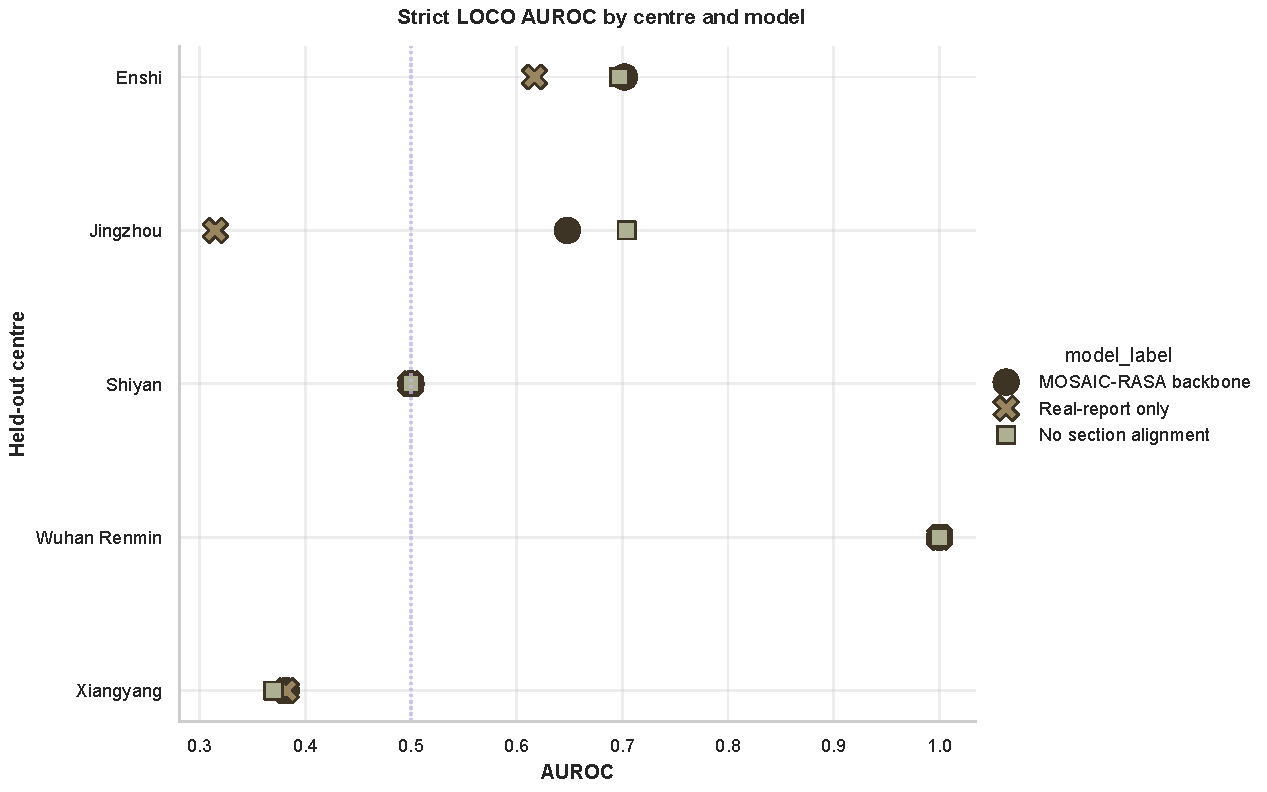
\includegraphics[width=\linewidth]{final_Fig/Figure4_loco_forest_catplot.pdf}
  \caption{Strict leave-one-centre-out behaviour under fixed quick-budget retraining. The centre-wise spread identifies residual distribution shift as a limitation of the current retrospective evidence.}
  \label{fig:loco_forest}
\end{figure}

Additional robustness and systems audits supported reproducible retrospective batch analysis. Multi-seed AUROC for the MOSAIC--RASA backbone was stable (mean 0.776; 95\% interval, 0.773--0.781; SD 0.004). Report-level safety summaries showed no missing-modality hallucination or section incompleteness in the evaluated settings, while the refreshed failure-enriched QC audit provided the primary evidence for contradiction, unsupported-terminology, missing-section, and duplicate-template detection. A case-level embedding audit covered all 1,897 cases; case identifiers, hashed patient identifiers, and embedding paths did not cross splits, although repeated raw colposcopy paths within the same split were retained as a data-provenance caveat rather than treated as cross-split leakage. The pipeline processed 137,591 images, stored 5,691 embedding files using 47.349 MB, and produced publishable checkpoints of approximately 80 MB. These findings support MOSAIC as a reproducible retrospective semantic-prior analytics framework. Prospective validation, stronger centre-shift mitigation, expert review of generated report sections, and broader foundation-model benchmarking remain necessary before clinical utility can be claimed.

The eval-only LOCO table is retained separately because it answers a different question: how a global checkpoint behaves when evaluated by centre, rather than how the model performs after centre-held-out retraining. Similarly, the multi-seed, report-safety, masking-validation, and scalability summaries are treated as reproducibility and systems evidence. They support the feasibility of retrospective cohort-scale semantic-prior analysis, but they do not remove the need for prospective validation, predefined operating thresholds, expert review of generated sections, and domain-shift mitigation.

\FloatBarrier

Overall, the results form a coherent but bounded story. The cohort analysis demonstrates a centre-dependent report-supervision bottleneck. Phase O shows that QC-gated weak-oracle pseudo reports provide modality-grounded semantic supervision beyond label templates. Phase S shows relative section-wise organisation of multimodal representations. The scarcity analysis shows that pseudo-report augmentation is most valuable when real reports are limited. Finally, Phase A+I+C improves locked held-out prediction through train-only semantic retrieval and validation-calibrated fusion. The same results also set the manuscript boundary: MOSAIC is a leakage-controlled retrospective framework for LLM-augmented semantic-prior learning under incomplete report supervision. It is not an autonomous LLM diagnostic system, not a substitute for clinician-authored reports, and not yet a prospectively validated clinical tool.

% Supplementary Appendix Full Evidence Chain
\clearpage
\section{Supplementary Experiments and Results}
\label{sec:supplementary_experiments_results}

The main Results section reports the experimental story in prose and keeps the principal tables and figures needed to follow the MOSAIC argument. This appendix preserves the full submission evidence base, including S tables, provider-stage figures, ablation plots, perturbation plots, cross-centre analyses, masking validation, safety summaries, and scalability checks. These supplementary materials should be read as audit evidence. They support the retrospective semantic-prior framework, but they do not establish autonomous LLM diagnosis, replacement of clinician-authored reports, or prospective clinical deployment.

\subsection{Supplementary weak-oracle generation and provider audit}
These tables and figures preserve the Phase O details: clean pseudo-report feasibility, provider-level quality, operational reliability, and staged API analyses. Provider results are auxiliary implementation audits and do not define the default MOSAIC training source.

\begin{table*}[!htbp]
  \centering
  \caption{Supplementary LLM provider comparison for structured pseudo-report generation.}
  \label{tab:llm_provider_comparison}
  \scriptsize
  \begin{threeparttable}
  \resizebox{\linewidth}{!}{%
  \begin{tabular}{lrrrrrrr}
    \toprule
    \textbf{Source} & \textbf{Valid/req.} & \textbf{Section comp.} & \textbf{Modality supp.} & \textbf{Contradiction rate} & \textbf{Duplicate frac.} & \textbf{Alignment MRR} & \textbf{Latency (s)} \\
    \midrule
    Template              & 100/100 & 1.000 & 0.000 & \textbf{0.000} & 0.860 & 0.110 & N/A \\
    Rule-based            & 100/100 & 1.000 & 1.000 & \underline{0.040} & \textbf{0.010} & 0.102 & N/A \\
    Local embedding LLM   & 100/100 & 1.000 & 1.000 & \underline{0.040} & \textbf{0.010} & 0.098 & N/A \\
    Qwen-Plus             & 10/10   & 1.000 & 1.000 & 0.600 & 0.100 & \underline{0.318} & 13.68 \\
    GLM-4.7-Flash         & 10/10   & 1.000 & 0.933 & 0.300 & 0.100 & 0.295 & 25.06 \\
    Gemini-3.1-Pro        & 9/9     & 1.000 & 1.000 & 0.444 & 0.111 & \textbf{0.366} & 25.70 \\
    GPT-5.5               & 100/100 & 0.810 & 0.810 & 0.050 & 0.190 & 0.063 & \textbf{11.39} \\
    \bottomrule
  \end{tabular}%
  }
  \begin{tablenotes}[flushleft]
    \footnotesize
    \item Schema-valid rate was 1.000 and hallucination rate was 0.000 for all evaluated sources; these non-informative duplicate rows were omitted from the body of the table. Latency was measured only for API providers. GPT-5.5 had an estimated cost of US\$27.73 per 1,000 cases. Qwen-Plus, GLM-4.7-Flash, and Gemini-3.1-Pro were pilot cohorts; GPT-5.5 was the extended 100-case API cohort.
  \end{tablenotes}
  \end{threeparttable}
\end{table*}

\begin{table}[!htbp]
  \centering
  \caption{Supplementary Table S8. LLM pseudo-report quality-control summary.}
  \label{tab:s8_llm_pseudo_report_qc}
  \small
  \begin{threeparttable}
  \begin{tabular}{lrr}
    \toprule
    \textbf{Source} & \textbf{$n$} & \textbf{Pass rate} \\
    \midrule
    Mock pseudo reports & 1,153 & 1.000 \\
    LLM pseudo reports  & 1,153 & 1.000 \\
    \bottomrule
  \end{tabular}
  \begin{tablenotes}[flushleft]
    \footnotesize
    \item Invalid placeholder entries and duplicated source-table metadata were removed. The quality-summary row also contained $n_{\mathrm{QC}}=1,153$ and pass rate = 1.000.
  \end{tablenotes}
  \end{threeparttable}
\end{table}

\begin{figure}[!htbp]
  \centering
  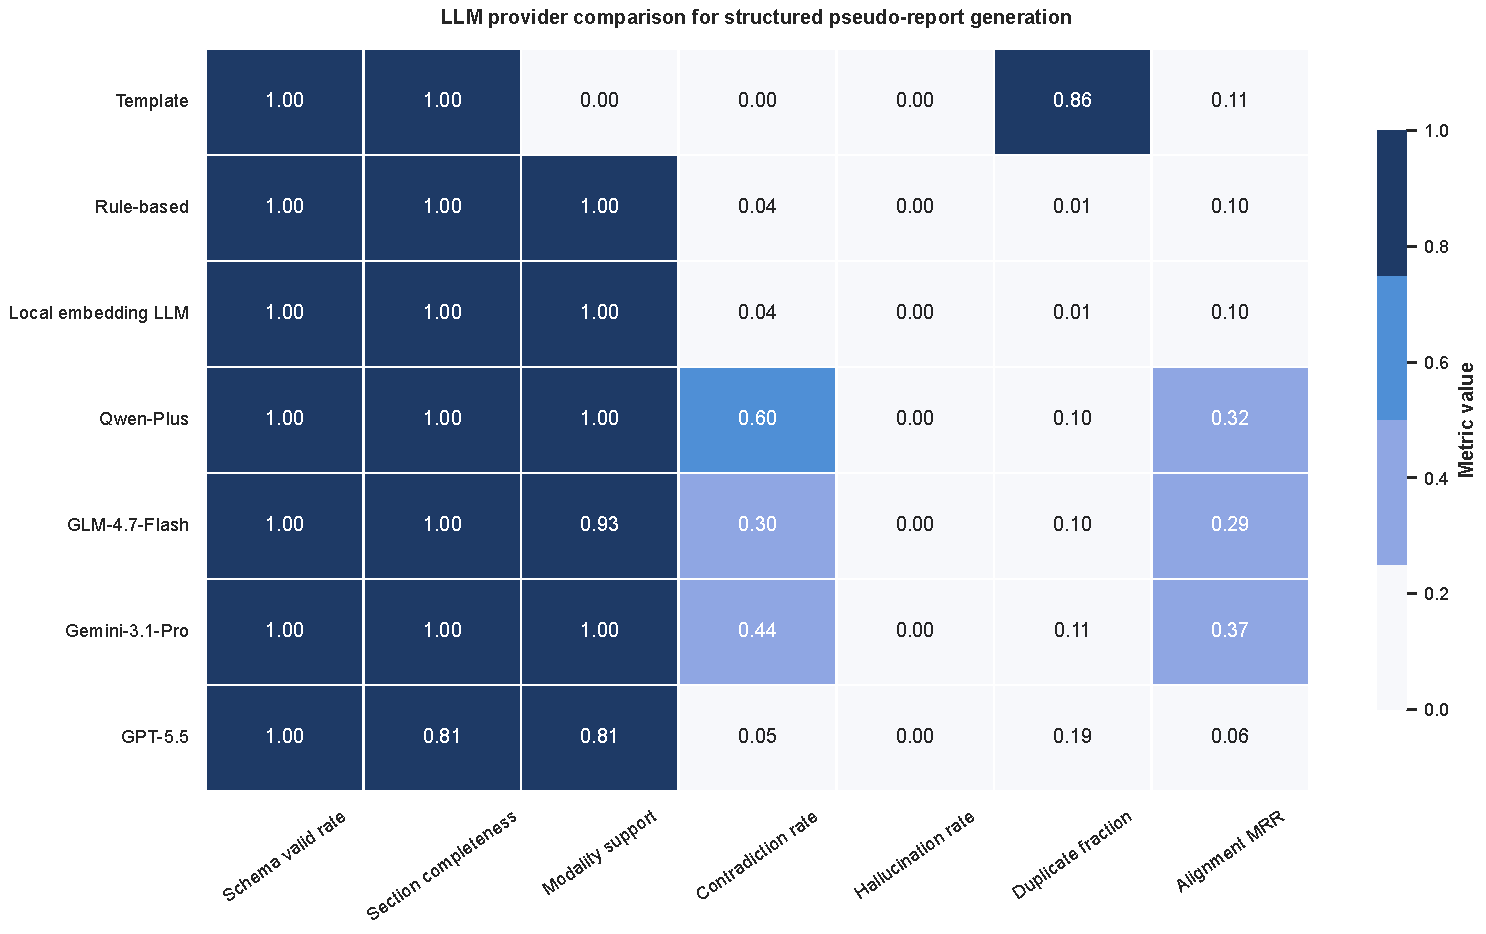
\includegraphics[width=\linewidth]{final_Fig/P8_llm_provider_comparison_heatmap.pdf}
  \caption{Supplementary provider-level comparison for structured pseudo-report generation. The heatmap summarises schema adherence, section completeness, modality support, contradiction risk, duplication, alignment, latency, and cost across template, rule-based, local LLM, and external API-based sources.}
  \label{fig:api_provider_summary_heatmap}
\end{figure}

\begin{figure}[!htbp]
  \centering
  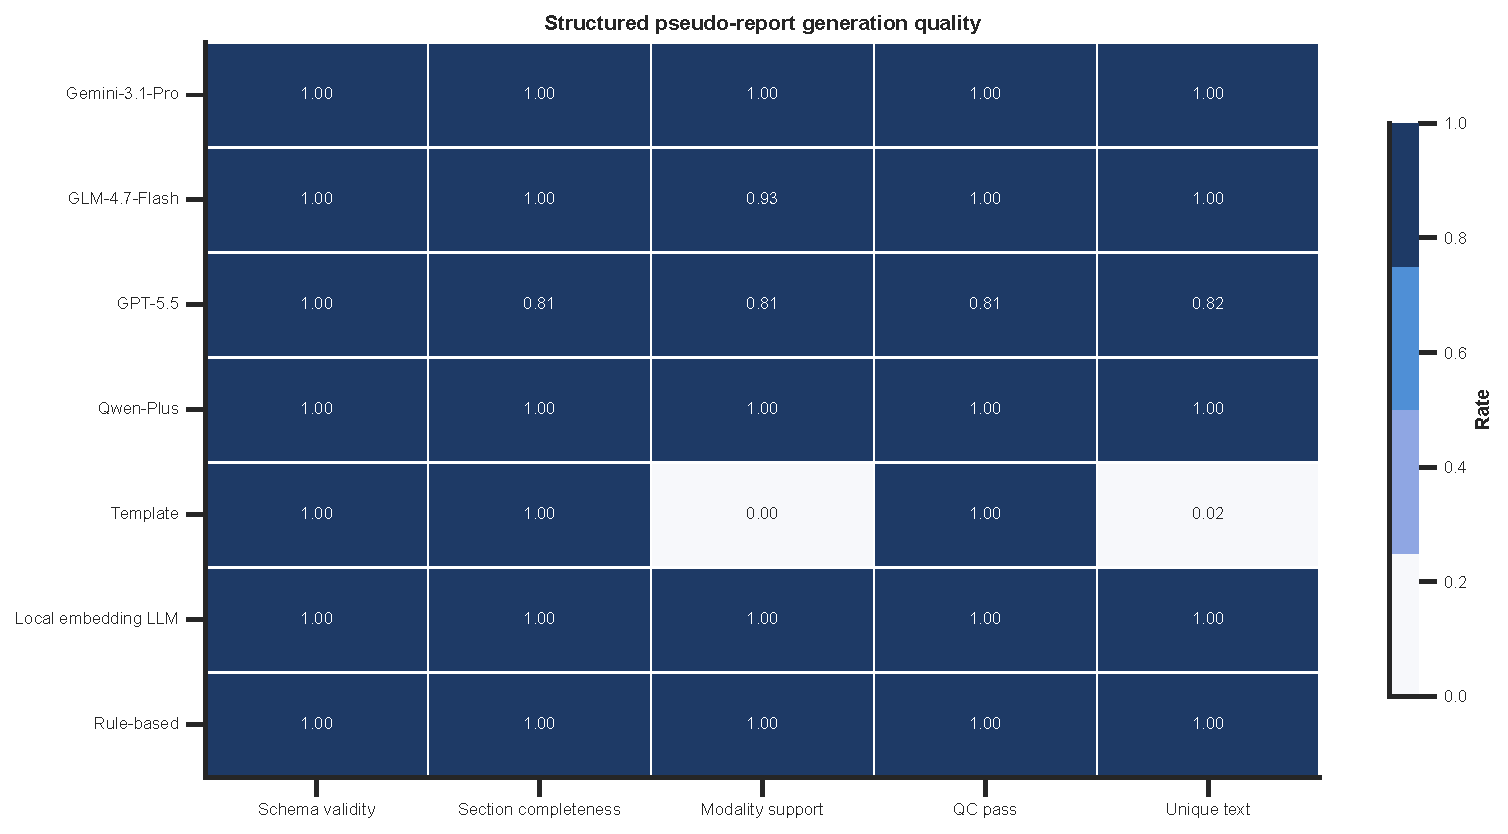
\includegraphics[width=\linewidth]{final_Fig/P1_stage1_quality_heatmap.pdf}
  \hfill
  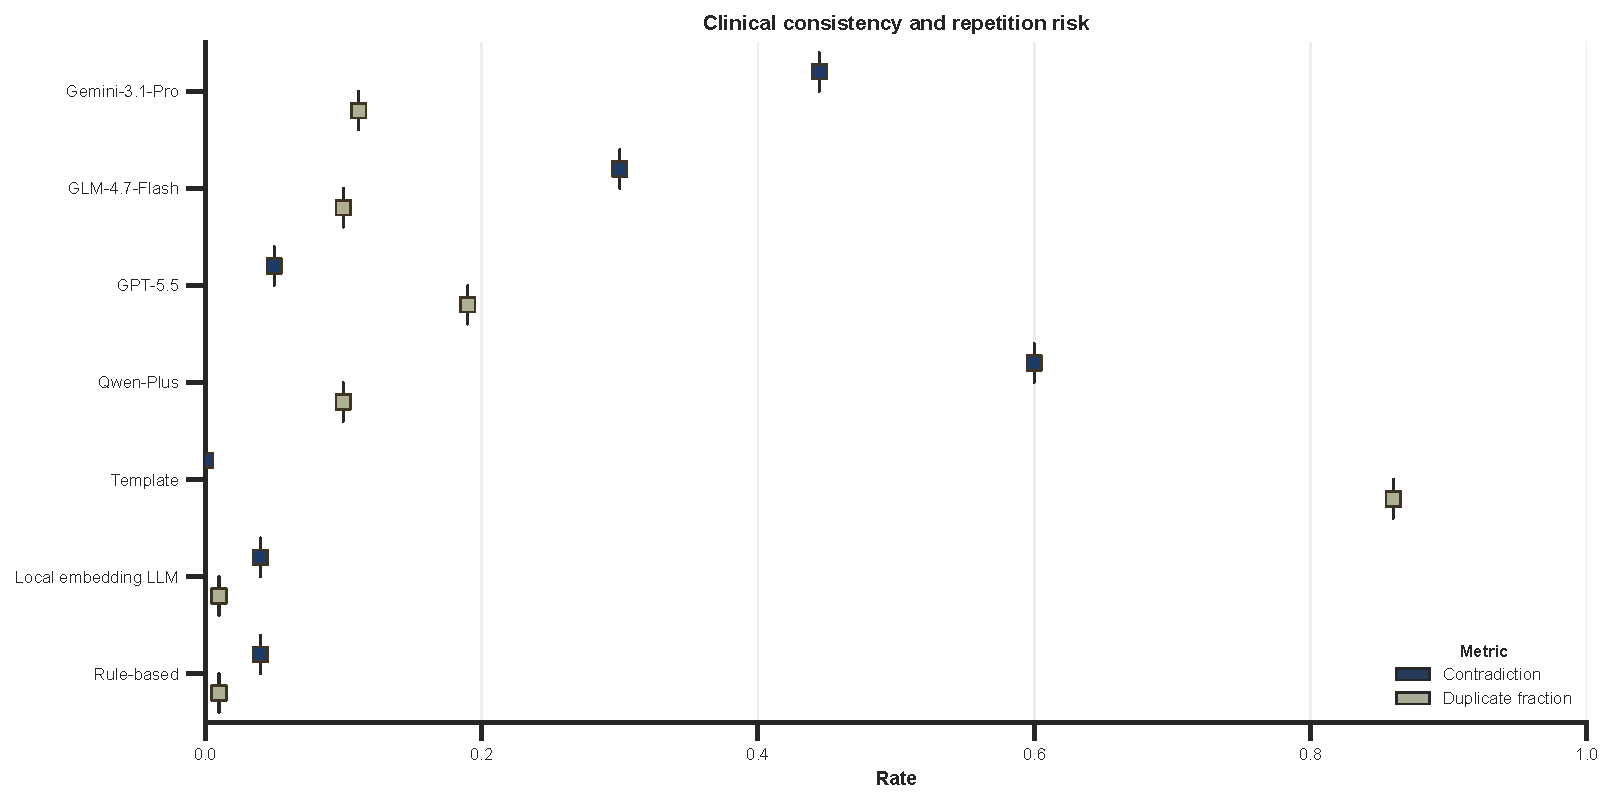
\includegraphics[width=\linewidth]{final_Fig/P2_stage1_quality_risk_bars.pdf}
  \caption{Supplementary Stage 1 evaluation of pseudo-report generation quality across LLM providers. The panels summarise generation validity and completeness together with risk-oriented quality indicators, including modality support, contradiction rate, hallucination rate, and duplicate-text behaviour.}
  \label{fig:api_quality_heatmap}
\end{figure}

\begin{figure}[!htbp]
  \centering
  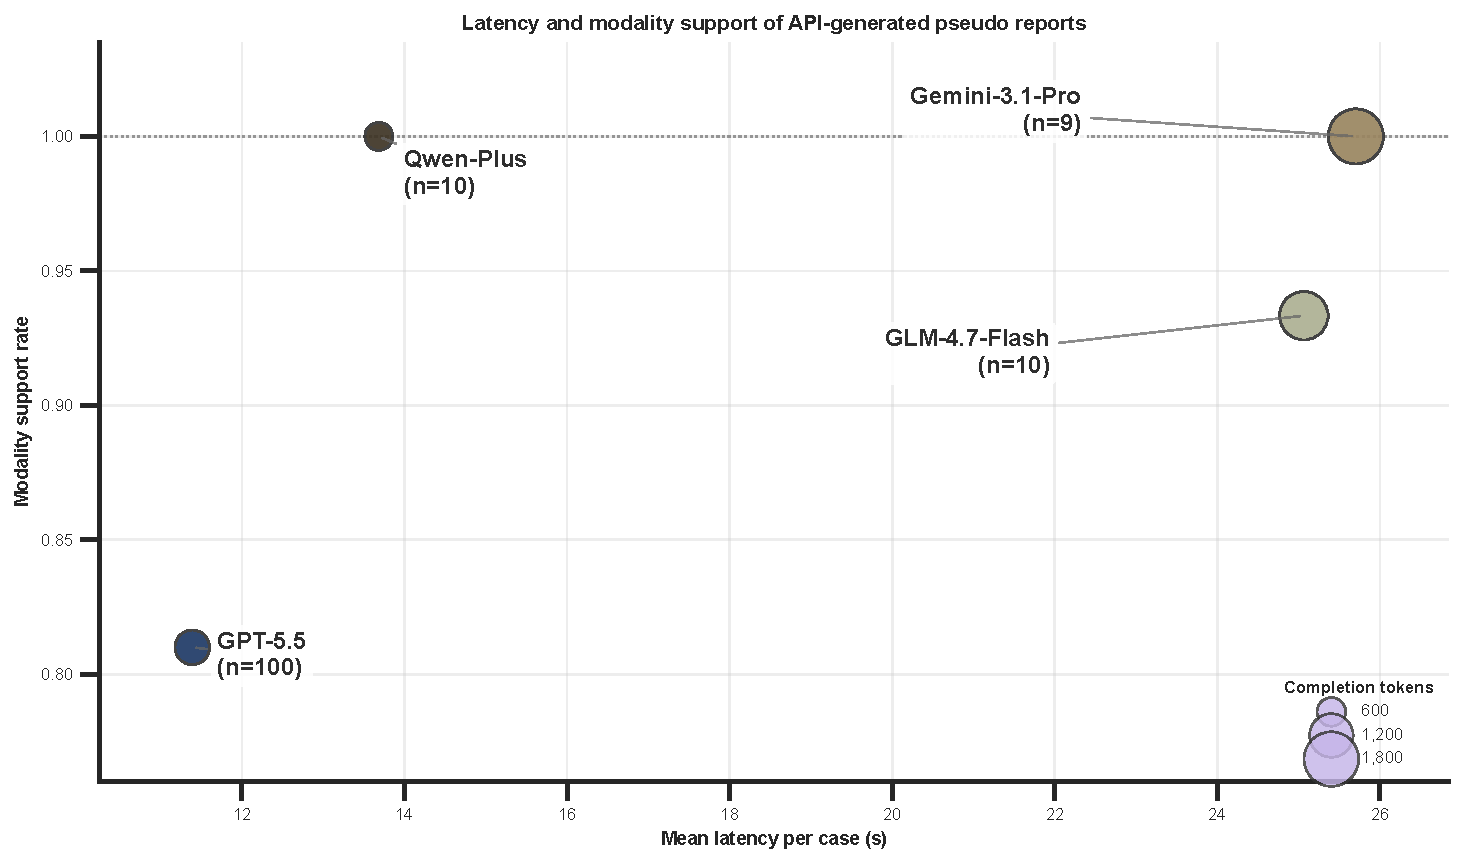
\includegraphics[width=\linewidth]{final_Fig/P3_stage1_latency_support_scatter.pdf}
  \hfill
  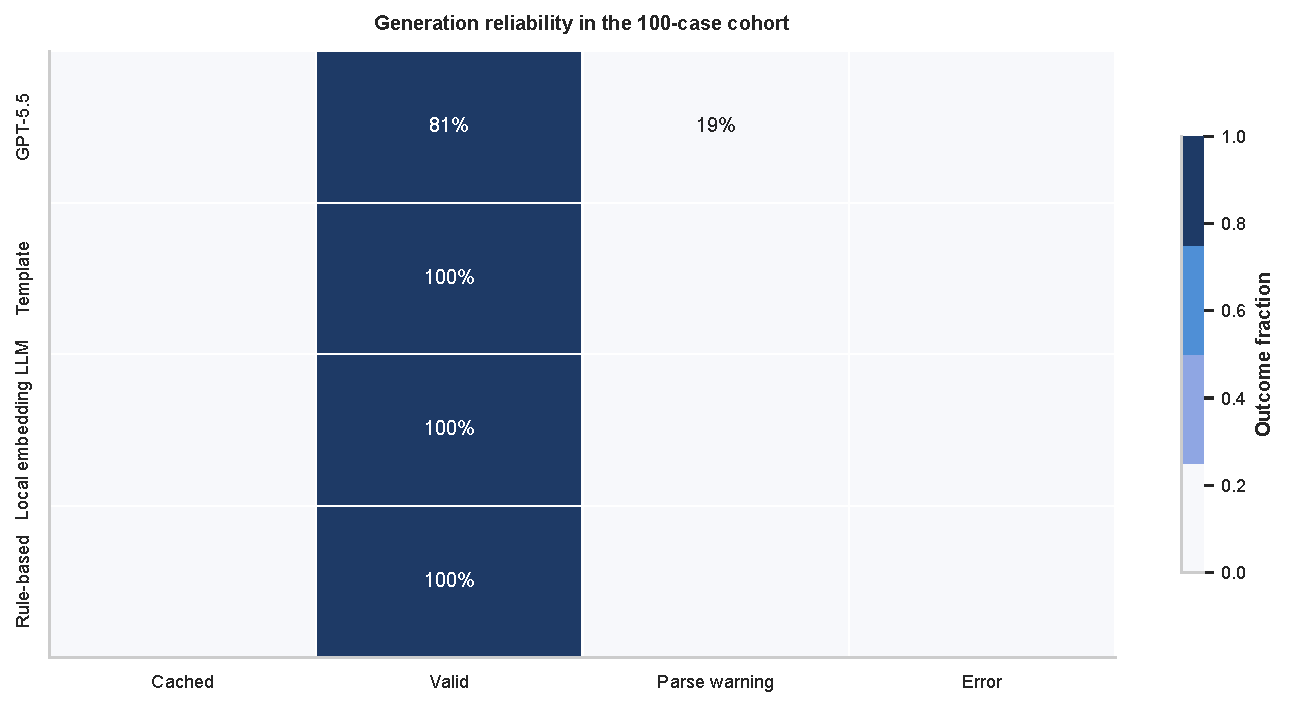
\includegraphics[width=\linewidth]{final_Fig/P4_stage1_generation_reliability.pdf}
  \caption{Supplementary operational reliability of external pseudo-report generation. The panels relate generation latency to modality support and summarise request completion and schema-valid output rates across evaluated providers.}
  \label{fig:api_reliability}
\end{figure}

\subsection{Supplementary section-alignment and scarcity analyses}
These figures retain the individual alignment, provider-alignment, and scarcity plots that support the mechanism narrative in the main text.

\begin{figure}[!htbp]
  \centering
  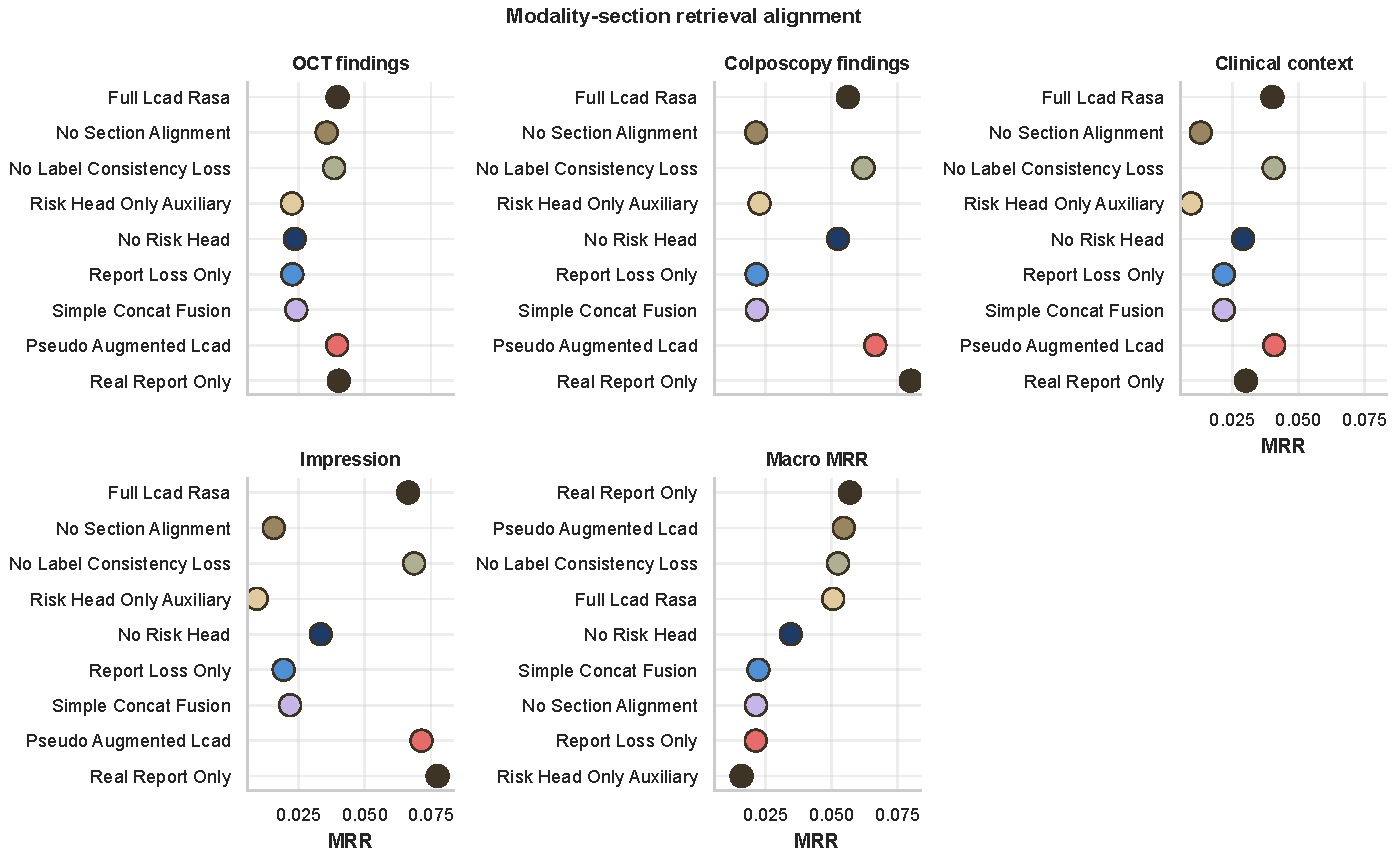
\includegraphics[width=\linewidth]{final_Fig/Figure_theme1_alignment_retrieval_mrr.pdf}
  \caption{Modality-section retrieval analysis for cross-modal semantic alignment under the retrospective protocol. Mean reciprocal rank quantifies whether modality-specific representations preferentially retrieve their corresponding report sections, providing a direct measure of section-wise alignment.}
  \label{fig:alignment_retrieval_mrr}
\end{figure}

\begin{figure}[!htbp]
  \centering
  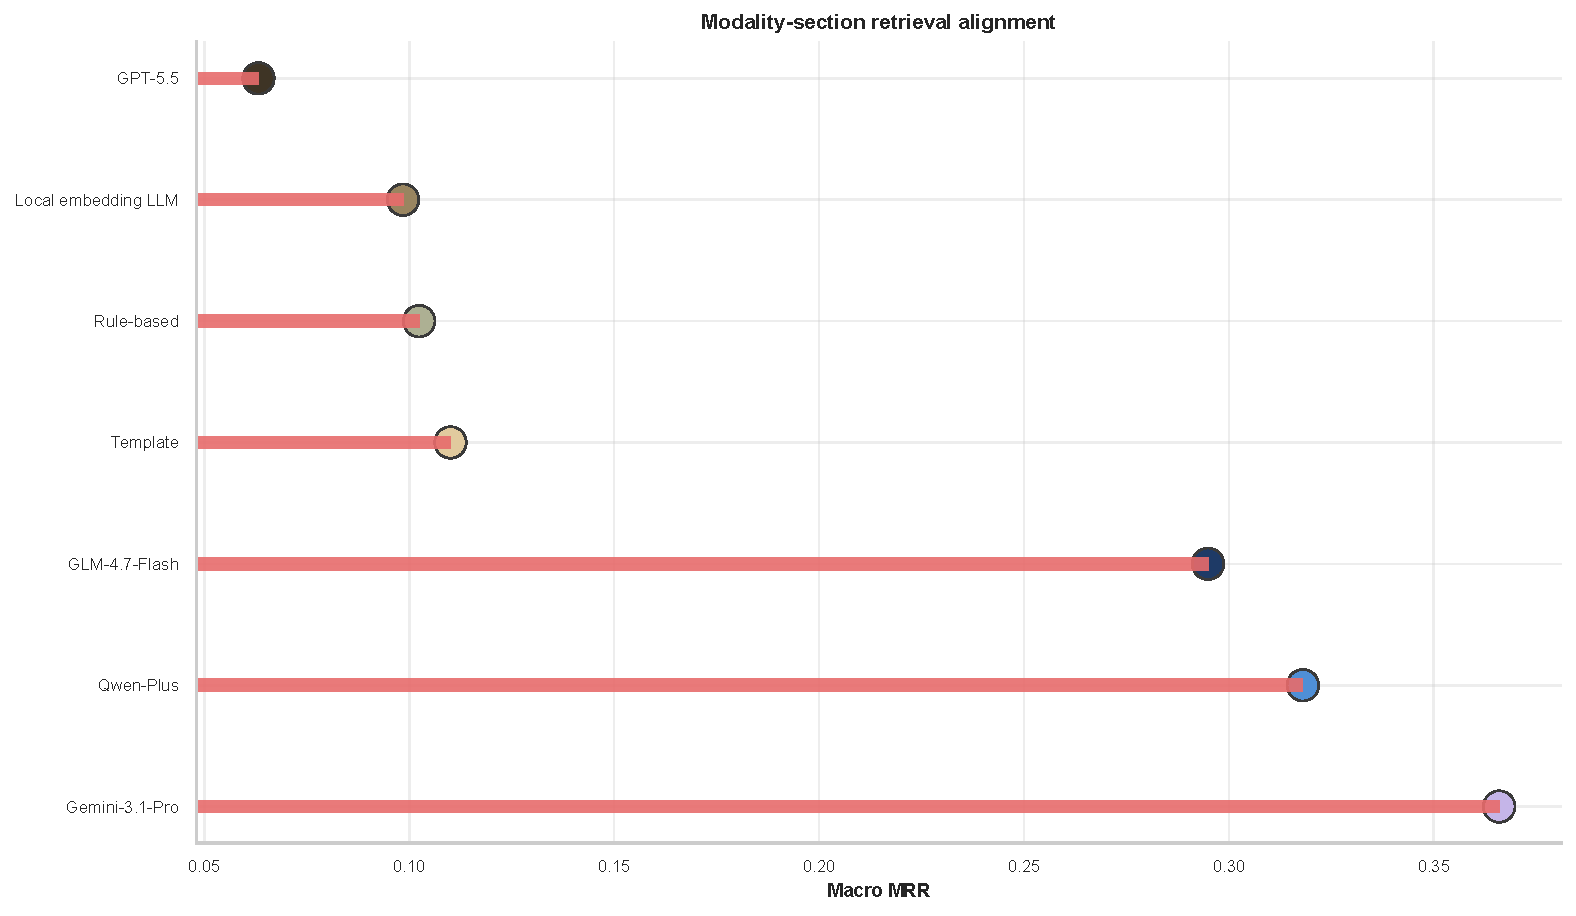
\includegraphics[width=\linewidth]{final_Fig/P5_stage2_macro_mrr.pdf}
  \hfill
  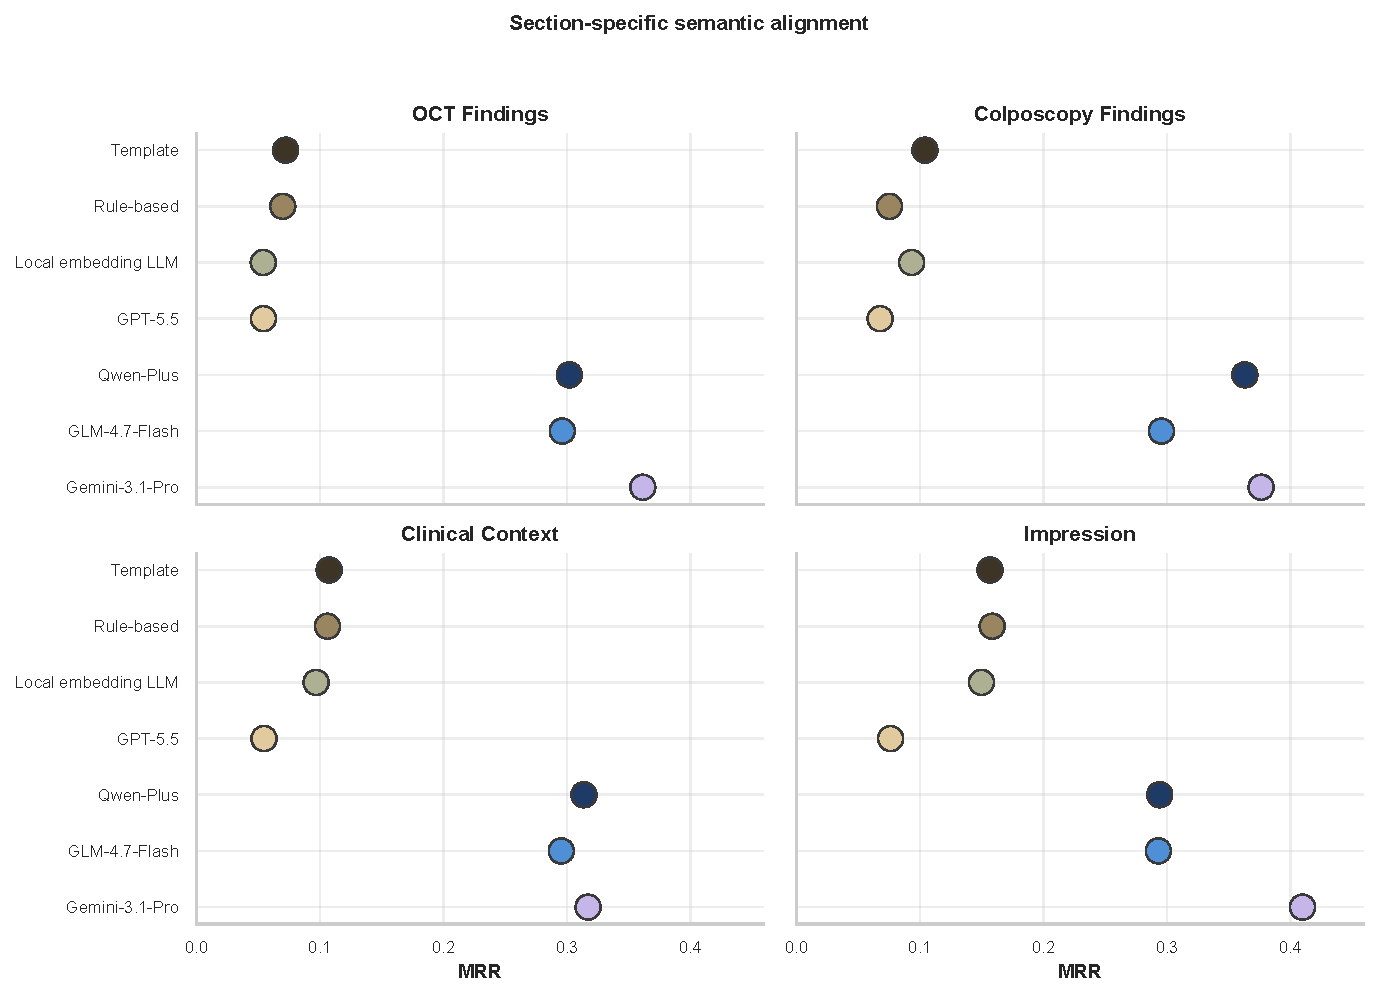
\includegraphics[width=\linewidth]{final_Fig/P6_stage2_section_mrr.pdf}
  \caption{Supplementary Stage 2 alignment evaluation for provider-generated pseudo reports. Macro MRR and section-specific MRR quantify how well report sections generated by different sources support modality-section semantic retrieval.}
  \label{fig:api_alignment_mrr}
\end{figure}

\begin{figure}[!htbp]
  \centering
  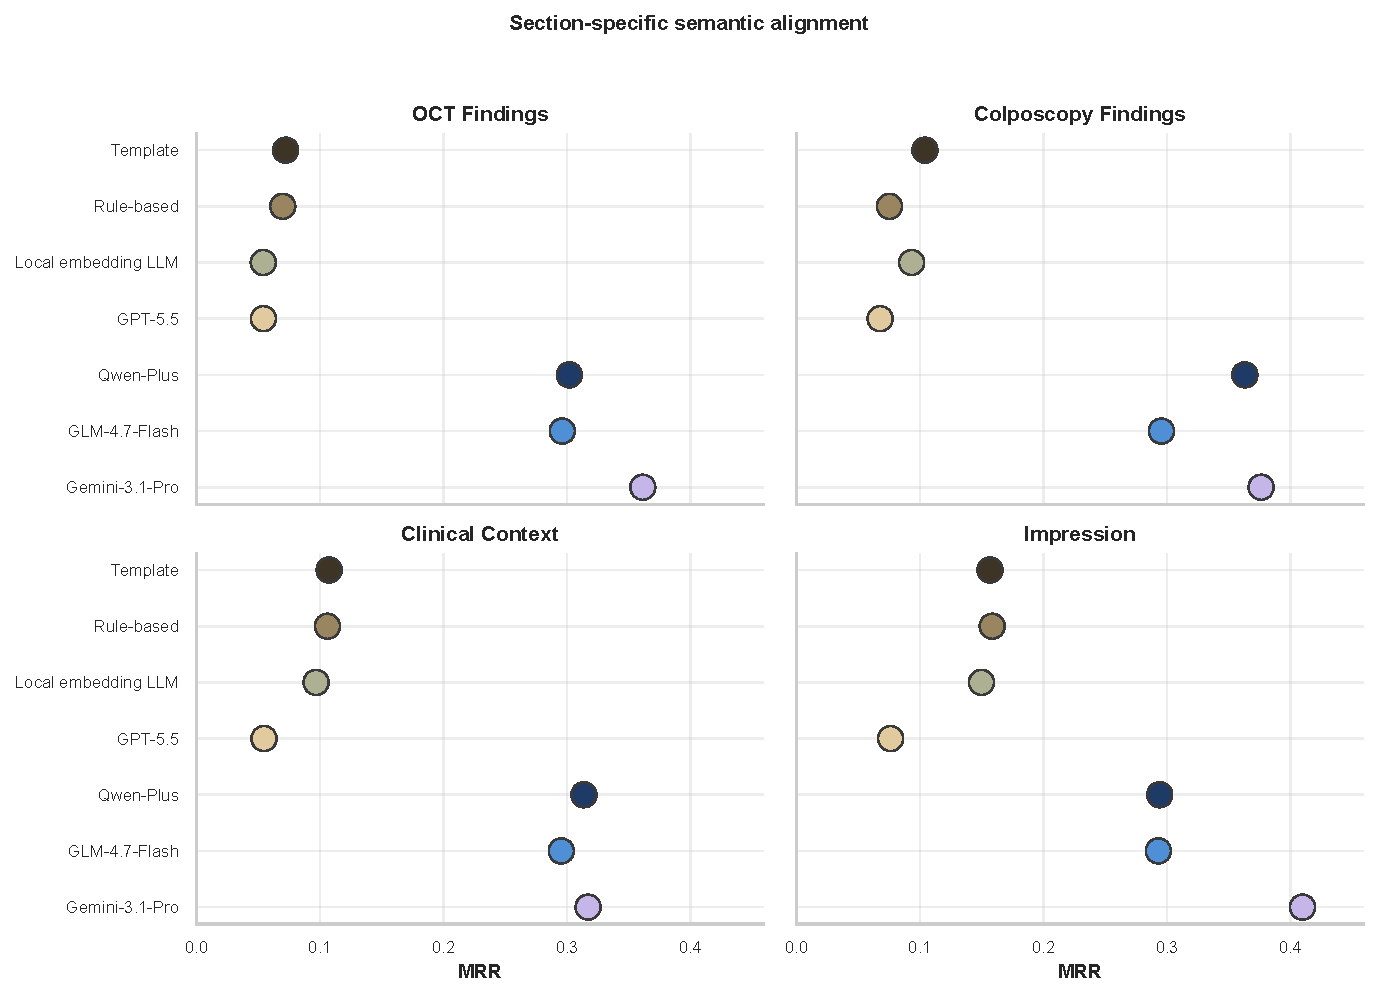
\includegraphics[width=\linewidth]{final_Fig/P6_stage2_section_mrr.pdf}
  \caption{Supplementary section-specific retrieval performance across pseudo-report providers. The analysis separately evaluates alignment for OCT findings, colposcopy findings, clinical context, and impression sections.}
  \label{fig:api_section_mrr}
\end{figure}

\begin{figure}[!htbp]
  \centering
  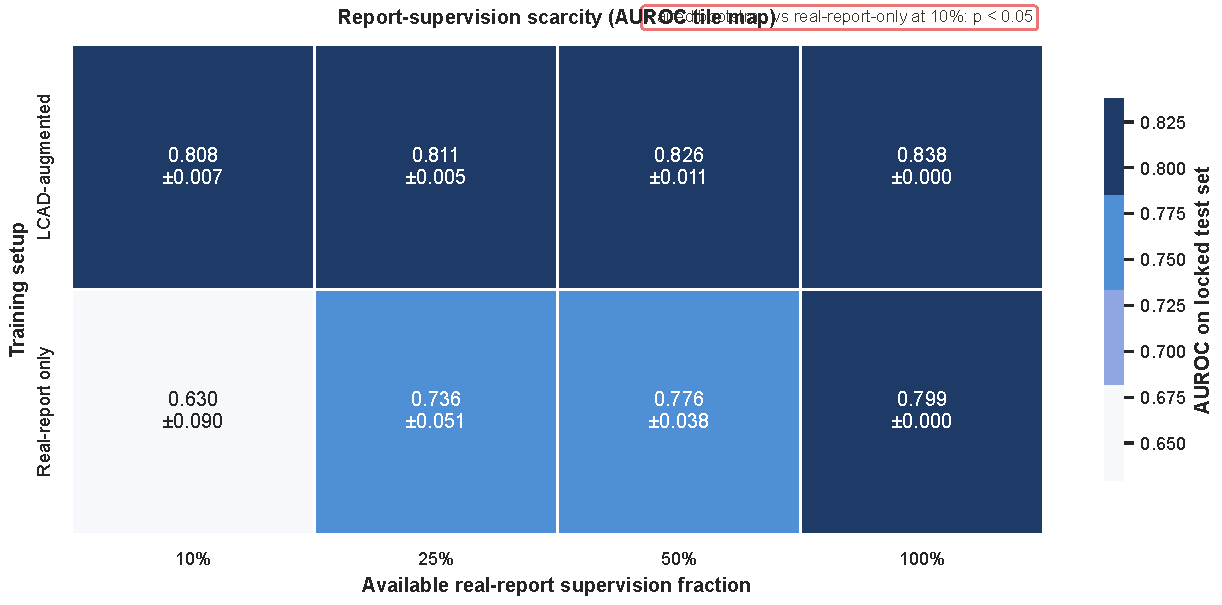
\includegraphics[width=\linewidth]{final_Fig/Figure_theme1_report_supervision_scarcity_curve.pdf}
  \caption{Effect of report-supervision scarcity on downstream surrogate performance under the retrospective scarcity protocol. AUROC and F1 are compared between real-report-only learning and pseudo-report-augmented learning as the proportion of available clinician-authored reports is progressively reduced.}
  \label{fig:scarcity_curve}
\end{figure}

\begin{figure}[!htbp]
  \centering
  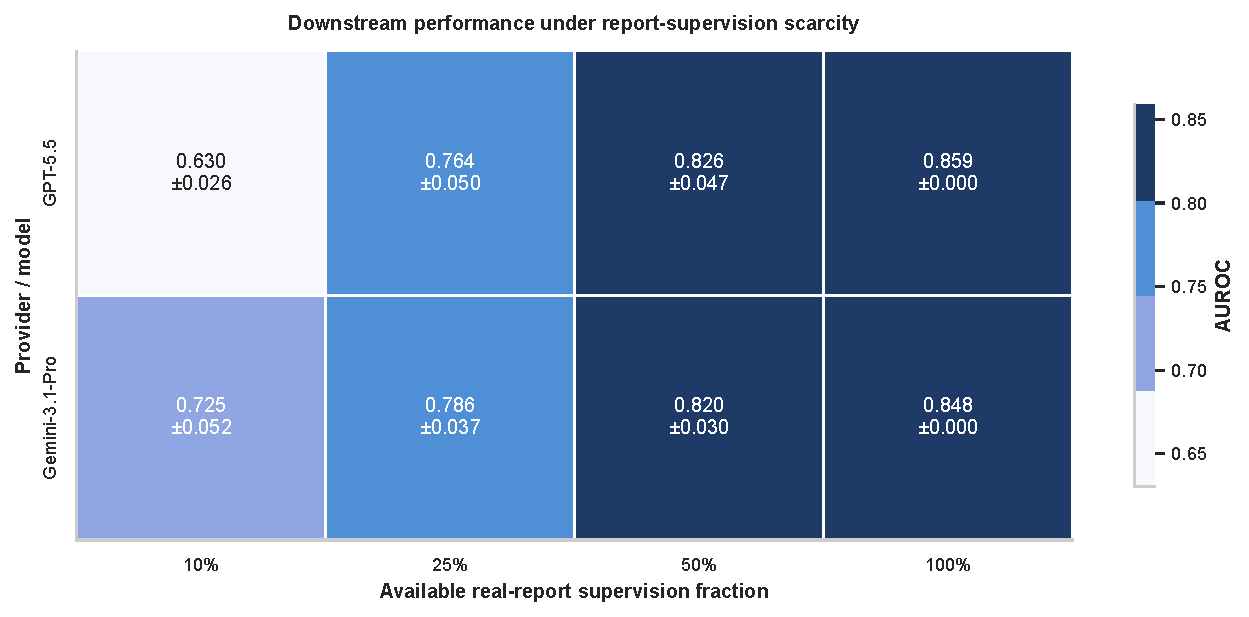
\includegraphics[width=\linewidth]{final_Fig/P7_stage3_scarcity_auc.pdf}
  \caption{Supplementary Stage 3 downstream scarcity surrogate using selected API-generated pseudo reports. The figure compares performance under reduced real-report supervision and evaluates whether externally generated structured reports provide useful supervision in low-report regimes.}
  \label{fig:api_scarcity_auc}
\end{figure}

\subsection{Supplementary protocol-harmonisation and historical backbone comparisons}
These outputs document the pre-retrieval LCAD--RASA experiment stack and show why the final manuscript distinguishes the MOSAIC--RASA backbone from the full retrieval-calibrated MOSAIC pipeline.

\begin{table*}[!htbp]
  \centering
  \caption{Supplementary protocol-harmonisation table. Pre-retrieval-calibration held-out test performance at validation-selected thresholds.}
  \label{tab:main_comparison}
  \scriptsize
  \begin{threeparttable}
  \resizebox{\linewidth}{!}{%
  \begin{tabular}{lrrr}
    \toprule
    \textbf{Model} & \textbf{AUROC [95\% CI]} & \textbf{F1 [95\% CI]} & \textbf{Threshold} \\
    \midrule
    \textbf{MOSAIC-RASA backbone} & \textbf{0.832} [0.757, 0.897] & \textbf{0.611} [0.458, 0.737] & 0.37 \\
    LCAD w/o section alignment     & \underline{0.826} [0.749, 0.894] & 0.510 [0.381, 0.624] & 0.24 \\
    Pseudo-augmented LCAD          & \underline{0.826} [0.747, 0.894] & \underline{0.545} [0.395, 0.674] & 0.39 \\
    Fusion w/o report anchor       & 0.802 [0.726, 0.873] & 0.457 [0.344, 0.557] & 0.16 \\
    Image-only report generator    & 0.763 [0.685, 0.837] & 0.453 [0.339, 0.553] & 0.17 \\
    Real-report only               & 0.725 [0.640, 0.801] & 0.356 [0.263, 0.438] & 0.14 \\
    Simple concatenation fusion    & 0.672 [0.584, 0.763] & 0.465 [0.380, 0.550] & 0.05 \\
    Instruction-only report generator & 0.630 [0.547, 0.717] & 0.459 [0.394, 0.519] & 0.14 \\
    \bottomrule
  \end{tabular}%
  }
  \begin{tablenotes}[flushleft]
    \footnotesize
    \item All models were evaluated on the same locked held-out test set ($n=288$). The repeated $n$ column was removed and reported here.
  \end{tablenotes}
  \end{threeparttable}
\end{table*}

\begin{figure}[!htbp]
  \centering
  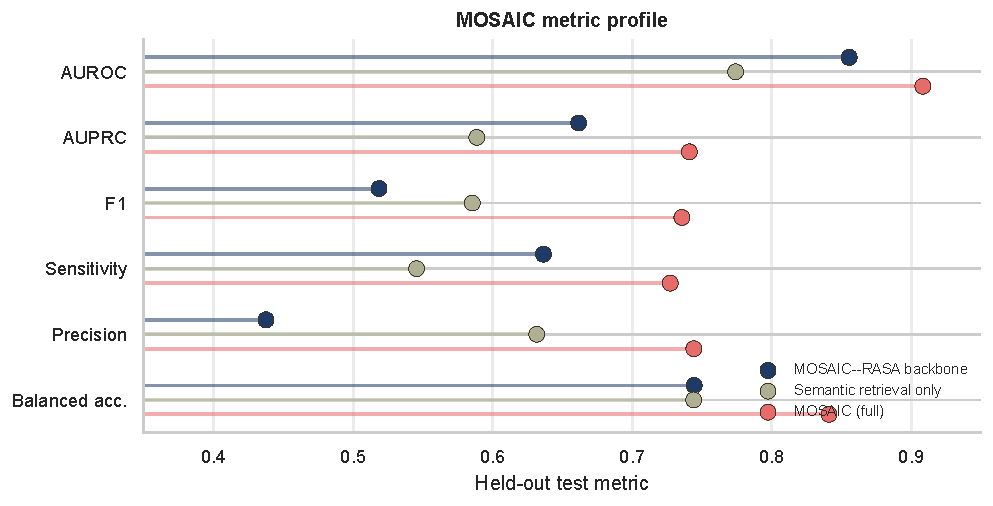
\includegraphics[width=\linewidth]{final_Fig/Figure_mosaic_metrics_heatmap.pdf}
  \caption{Supplementary compact metric heatmap for MOSAIC. The heatmap compares the MOSAIC-RASA backbone, retrieval-only semantic priors, and MOSAIC across discrimination and threshold-dependent metrics.}
  \label{fig:mosaic_metrics_heatmap}
\end{figure}

\begin{figure}[!htbp]
  \centering
  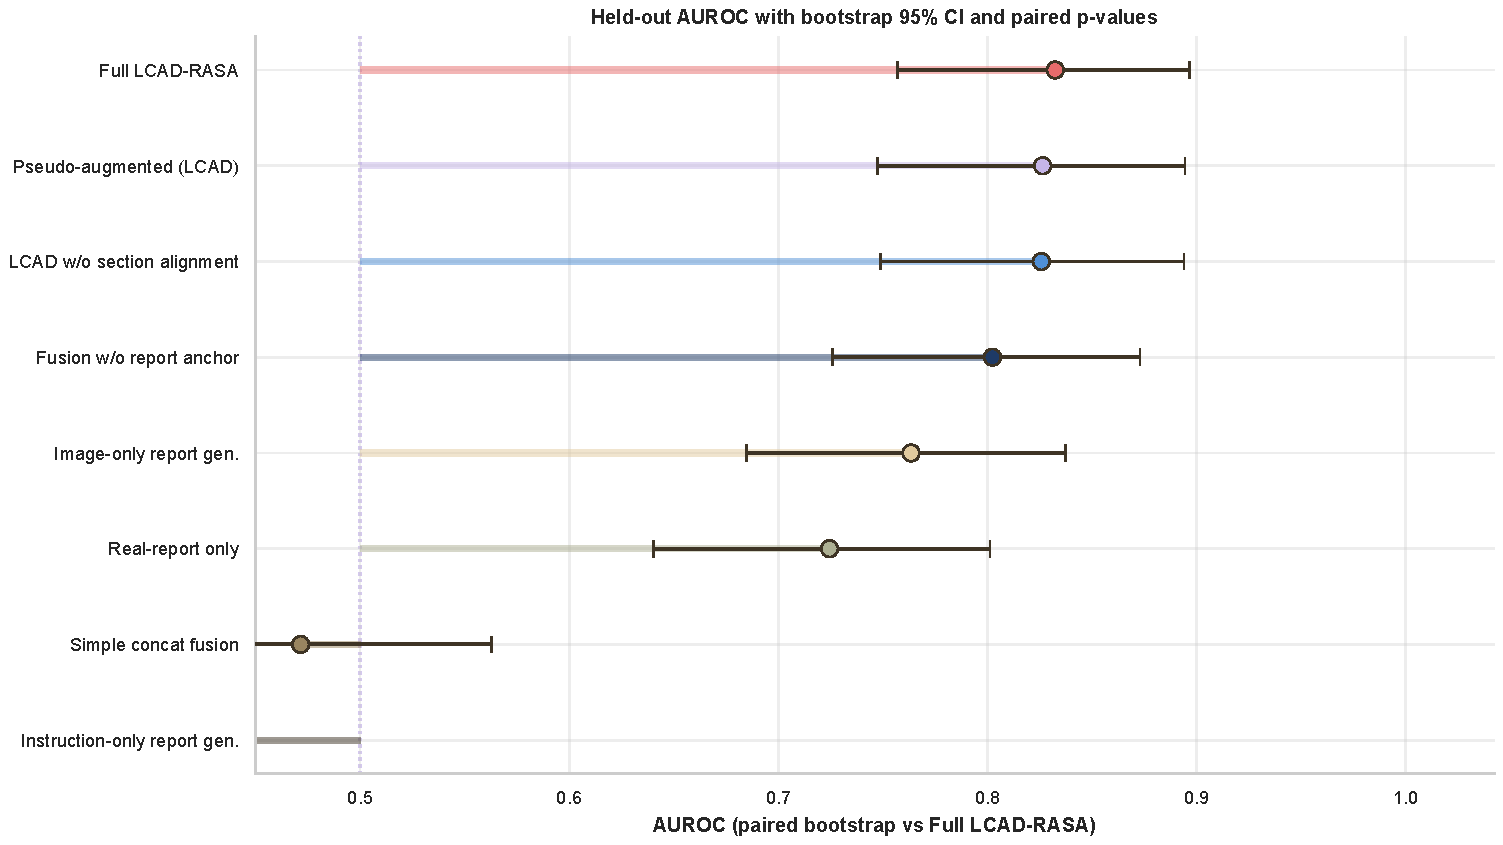
\includegraphics[width=\linewidth]{final_Fig/Figure_main_AUC_pointplot.pdf}
  \caption{Supplementary protocol-harmonisation plot. Held-out AUROC of report-aware backbone variants under the locked retrospective protocol. Points indicate test-set AUROC and intervals denote bootstrap 95\% confidence intervals.}
  \label{fig:main_auc}
\end{figure}

\begin{figure}[!htbp]
  \centering
  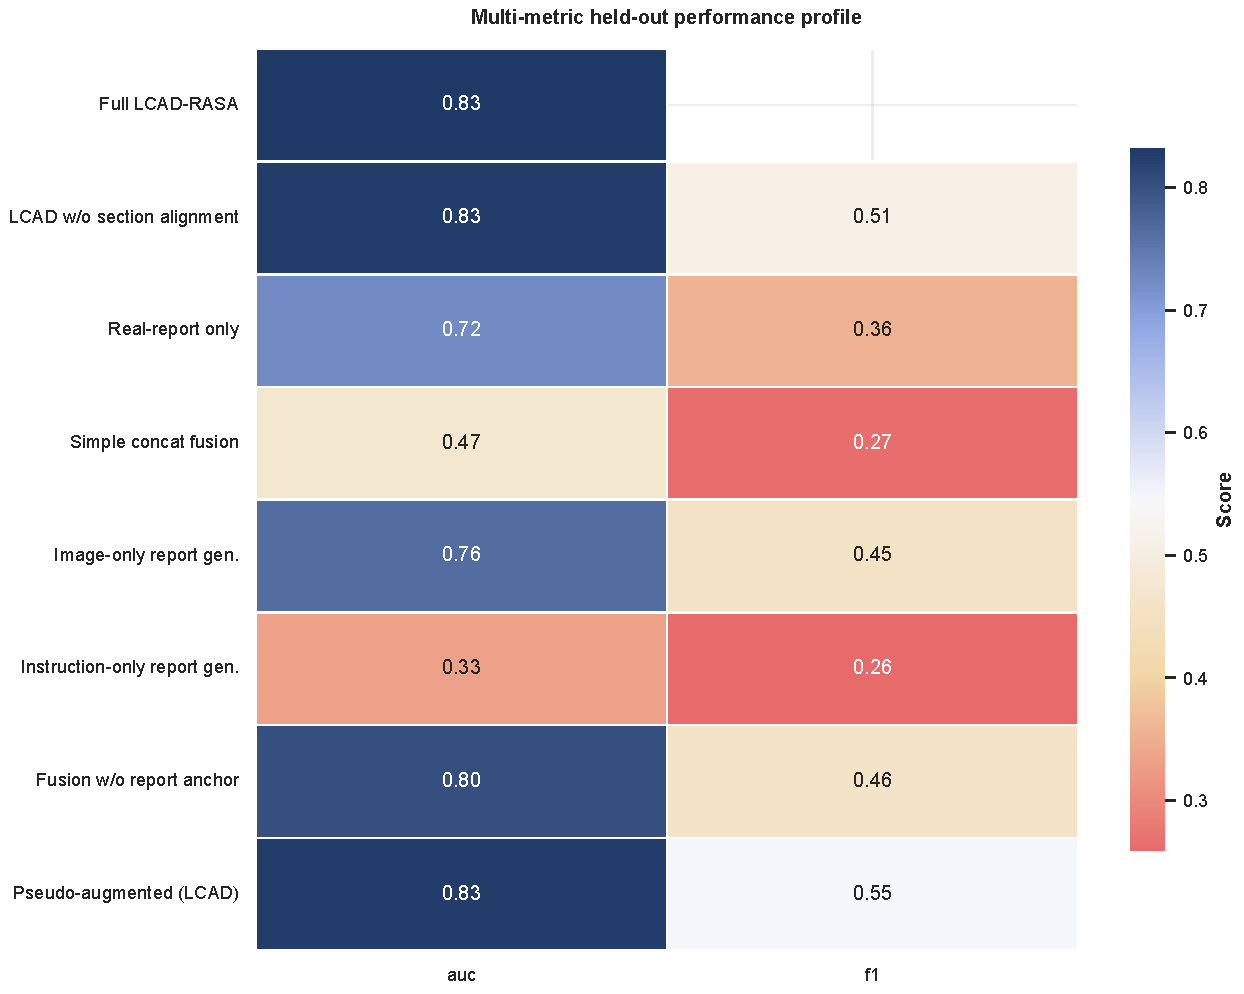
\includegraphics[width=\linewidth]{final_Fig/Figure_main_metrics_heatmap.pdf}
  \caption{Supplementary multi-metric held-out performance profile across historical backbone variants. The heatmap summarises discrimination, threshold-dependent performance, report consistency, and related evaluation metrics under the same locked test protocol.}
  \label{fig:main_metrics}
\end{figure}

\begin{figure}[!htbp]
  \centering
  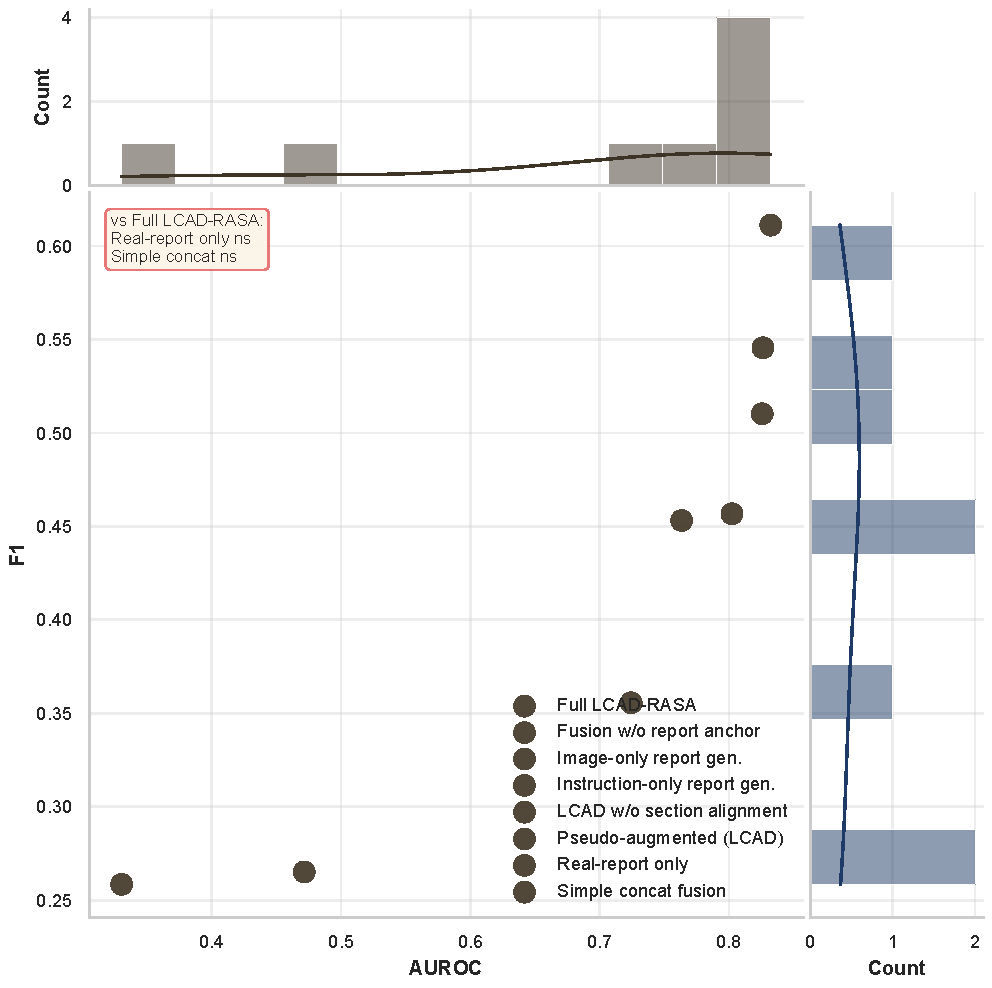
\includegraphics[width=\linewidth]{final_Fig/Figure_main_auc_f1_scatter.pdf}
  \caption{Supplementary AUROC--F1 operating trade-off across historical backbone variants. The scatter plot contrasts rank-based discrimination with threshold-dependent classification performance on the held-out test set.}
  \label{fig:main_auc_f1}
\end{figure}

\subsection{Supplementary semantic-tag, ablation, and QC evidence}
These tables and figures retain the detailed semantic-tag audit, negative controls, RASA alignment-weight sweep, modality ablations, component ablations, QC ablations, and baseline metric rechecks.

\begin{table*}[!htbp]
  \centering
  \caption{Supplementary Table S4a. LLM-specific semantic-tag and retrieval ablation.}
  \label{tab:llm_specific_ablation}
  \scriptsize
  \begin{threeparttable}
  \resizebox{\linewidth}{!}{%
  \begin{tabular}{lcccrrrrrrr}
    \toprule
    \textbf{Method} & \textbf{Uses LLM} & \textbf{\makecell{Train-only\\bank}} & \textbf{\makecell{Validation\\fusion}} & \textbf{AUROC} & \textbf{AUPRC} & \textbf{F1} & \textbf{Sensitivity} & \textbf{Specificity} & \textbf{$\alpha$} & \textbf{Threshold} \\
    \midrule
    MOSAIC-RASA backbone only & No & N/A & Threshold only & 0.856 & 0.662 & 0.519 & 0.636 & 0.852 & N/A & 0.39 \\
    Clean rule-tag retrieval only & No & Yes & Threshold only & 0.724 & 0.349 & 0.480 & 0.682 & 0.791 & N/A & 0.30 \\
    MOSAIC-Tag: RASA + clean rule-tag fusion & No & Yes & Yes & 0.878 & 0.695 & 0.556 & 0.568 & 0.914 & 0.10 & 0.40 \\
    LLM-tag retrieval only & Yes & Yes & Threshold only & N/A & N/A & N/A & N/A & N/A & N/A & N/A \\
    RASA + LLM-tag retrieval fusion & Yes & Yes & Yes & N/A & N/A & N/A & N/A & N/A & N/A & N/A \\
    RASA + LLM-tag fusion + verifier weighting & Yes & Yes & Yes & N/A & N/A & N/A & N/A & N/A & N/A & N/A \\
    MOSAIC & Indirect & Yes & Yes & 0.908 & 0.741 & 0.736 & 0.727 & 0.955 & N/A & 0.50 \\
    CLIP-style contrastive baseline & No & N/A & Threshold only & 0.888 & 0.739 & 0.640 & 0.545 & 0.971 & N/A & 0.79 \\
    \bottomrule
  \end{tabular}%
  }
  \begin{tablenotes}[flushleft]
    \footnotesize
    \item LLM-tag rows are unavailable because no valid LLM semantic tag table was generated in the current run. Rule-tag rows are deterministic fallback audits and must not be interpreted as LLM evidence. All available tag-retrieval rows used a cleaned training-only bank; fusion weights and thresholds were selected on validation data only. MOSAIC-Tag is a secondary semantic-tag audit rather than the primary MOSAIC model.
  \end{tablenotes}
  \end{threeparttable}
\end{table*}

\begin{table*}[!htbp]
  \centering
  \caption{Supplementary Table S4b. Cleaned semantic-tag source ablation and negative controls.}
  \label{tab:semantic_tag_source_ablation_cleaned}
  \scriptsize
  \begin{threeparttable}
  \resizebox{\linewidth}{!}{%
  \begin{tabular}{lrrrrp{4.2cm}}
    \toprule
    \textbf{Variant} & \textbf{\makecell{Retrieval-only\\AUROC}} & \textbf{\makecell{Fusion\\AUROC}} & \textbf{\(\Delta\)AUROC vs RASA} & \textbf{\makecell{95\% interval}} & \textbf{Interpretation} \\
    \midrule
    MOSAIC-Tag, all clean rule tags & 0.724 & 0.878 & 0.023 & 0.003--0.042 & Cleaned semantic-tag audit; secondary analysis \\
    No impression tags & 0.724 & 0.878 & 0.023 & 0.003--0.042 & No loss after removing impression-tag column \\
    No severity tags & 0.724 & 0.878 & 0.023 & 0.003--0.042 & No loss after removing severity-tag column \\
    No diagnostic terminology & 0.724 & 0.878 & 0.023 & 0.003--0.042 & Effect persisted after diagnostic-term removal \\
    Modality-only or visual-only tags & 0.500 & 0.856 & 0.000 & 0.000--0.000 & Collapsed to MOSAIC-RASA backbone \\
    Train-label prior only & 0.500 & 0.856 & 0.000 & 0.000--0.000 & Negative control did not improve over backbone \\
    Random tag query & 0.462 & 0.853 & -0.002 & -0.006--0.002 & Random-query negative control removed the tag gain \\
    Random train-label bank & 0.582 & 0.856 & 0.000 & 0.000--0.000 & Label-permutation control removed the tag gain \\
    Same-centre excluded retrieval & 0.628 & 0.864 & 0.008 & -0.003--0.019 & Cross-centre retrieval retained limited signal but was weaker \\
    \bottomrule
  \end{tabular}%
  }
  \begin{tablenotes}[flushleft]
    \footnotesize
    \item All rows used the semantic-tag audit protocol: cleaned tag input, training-only tag bank, validation-selected fusion weight and threshold, and locked held-out test metrics. MOSAIC-Tag passed leakage screening and negative controls, but its role is a lightweight semantic-prior audit rather than a replacement for MOSAIC.
  \end{tablenotes}
  \end{threeparttable}
\end{table*}

\begin{table}[!htbp]
  \centering
  \caption{Supplementary Table S1. RASA alignment-weight sweep.}
  \label{tab:s1_rasa_lambda_align_sweep}
  \small
  \begin{threeparttable}
  \begin{tabular}{lr}
    \toprule
    \textbf{$\lambda_{\mathrm{align}}$} & \textbf{AUROC} \\
    \midrule
    0.00 & 0.766 \\
    0.01 & 0.766 \\
    0.05 & 0.769 \\
    0.10 & 0.773 \\
    0.20 & \textbf{0.776} \\
    0.50 & 0.772 \\
    1.00 & 0.764 \\
    \bottomrule
  \end{tabular}
  \begin{tablenotes}[flushleft]
    \footnotesize
    \item F1 was 0.451, label consistency was 0.641, and section completeness was 1.000 for all settings; these constant columns were omitted.
  \end{tablenotes}
  \end{threeparttable}
\end{table}

\begin{table*}[!htbp]
  \centering
  \caption{Supplementary Table S3. Modality ablation.}
  \label{tab:s3_modality_ablation}
  \small
  \begin{threeparttable}
  \resizebox{\linewidth}{!}{%
  \begin{tabular}{lrrrr}
    \toprule
    \textbf{Variant} & \textbf{AUROC} & \textbf{F1} & \textbf{Sensitivity} & \textbf{Specificity} \\
    \midrule
    Colposcopy + clinical instruction        & \textbf{0.850} & 0.524 & \underline{0.614} & 0.869 \\
    Full without fused visual embedding      & \underline{0.840} & \underline{0.571} & 0.500 & \textbf{0.955} \\
    OCT + colposcopy + clinical instruction  & \underline{0.840} & \underline{0.571} & 0.500 & \textbf{0.955} \\
    Colposcopy only                          & 0.838 & \textbf{0.581} & \underline{0.614} & 0.910 \\
    Full with fused visual embedding         & 0.836 & 0.561 & 0.523 & 0.939 \\
    OCT + colposcopy                         & 0.826 & 0.543 & 0.568 & 0.906 \\
    OCT + clinical instruction               & 0.765 & 0.466 & 0.386 & \underline{0.951} \\
    OCT only                                 & 0.740 & 0.353 & 0.409 & 0.836 \\
    Clinical instruction only                & 0.683 & 0.441 & \textbf{0.727} & 0.717 \\
    \bottomrule
  \end{tabular}%
  }
  \begin{tablenotes}[flushleft]
    \footnotesize
    \item Label consistency was 0.641 for all modality variants and was removed as a constant column.
  \end{tablenotes}
  \end{threeparttable}
\end{table*}

\begin{table}[!htbp]
  \centering
  \caption{Supplementary Table S4. LCAD pseudo-report quality-control ablation.}
  \label{tab:s4_lcad_qc_ablation}
  \small
  \begin{threeparttable}
  \begin{tabular}{lrrrr}
    \toprule
    \textbf{QC strategy} & \textbf{AUROC} & \textbf{F1} & \textbf{Sensitivity} & \textbf{Specificity} \\
    \midrule
    \makecell[l]{Pseudo reports, no QC;\\QC-pass pseudo reports only;\\QC-score weighting only;\\Pseudo confidence weighting only;\\QC-confidence weighted pseudo reports} & 0.836 & 0.561 & 0.523 & 0.939 \\
    \bottomrule
  \end{tabular}
  \begin{tablenotes}[flushleft]
    \footnotesize
    \item All QC variants produced identical downstream metrics under this retrospective configuration. Duplicate rows were therefore merged. Label consistency was 0.641 for all variants.
  \end{tablenotes}
  \end{threeparttable}
\end{table}

\begin{table*}[!htbp]
  \centering
  \caption{Supplementary Table S5. RASA component ablation.}
  \label{tab:s5_rasa_component_ablation}
  \small
  \begin{threeparttable}
  \resizebox{\linewidth}{!}{%
  \begin{tabular}{lrrrr}
    \toprule
    \textbf{Variant} & \textbf{AUROC} & \textbf{F1} & \textbf{Sensitivity} & \textbf{Specificity} \\
    \midrule
    Risk-head auxiliary only                 & \textbf{0.838} & 0.538 & \underline{0.568} & 0.902 \\
    No section alignment                     & \textbf{0.838} & 0.479 & \textbf{0.636} & 0.816 \\
    No label-consistency loss                & 0.836 & \textbf{0.579} & 0.500 & \textbf{0.959} \\
    MOSAIC-RASA backbone                    & 0.836 & \underline{0.561} & 0.523 & \underline{0.939} \\
    \makecell[l]{No risk head;\\Report loss only;\\Section alignment auxiliary only} & 0.750 & 0.465 & 0.550 & 0.820 \\
    \bottomrule
  \end{tabular}%
  }
  \begin{tablenotes}[flushleft]
    \footnotesize
    \item Label consistency was 0.641 for all component variants and was removed as a constant column. Three variants with identical metrics were merged into one row.
  \end{tablenotes}
  \end{threeparttable}
\end{table*}

\begin{figure}[!htbp]
  \centering
  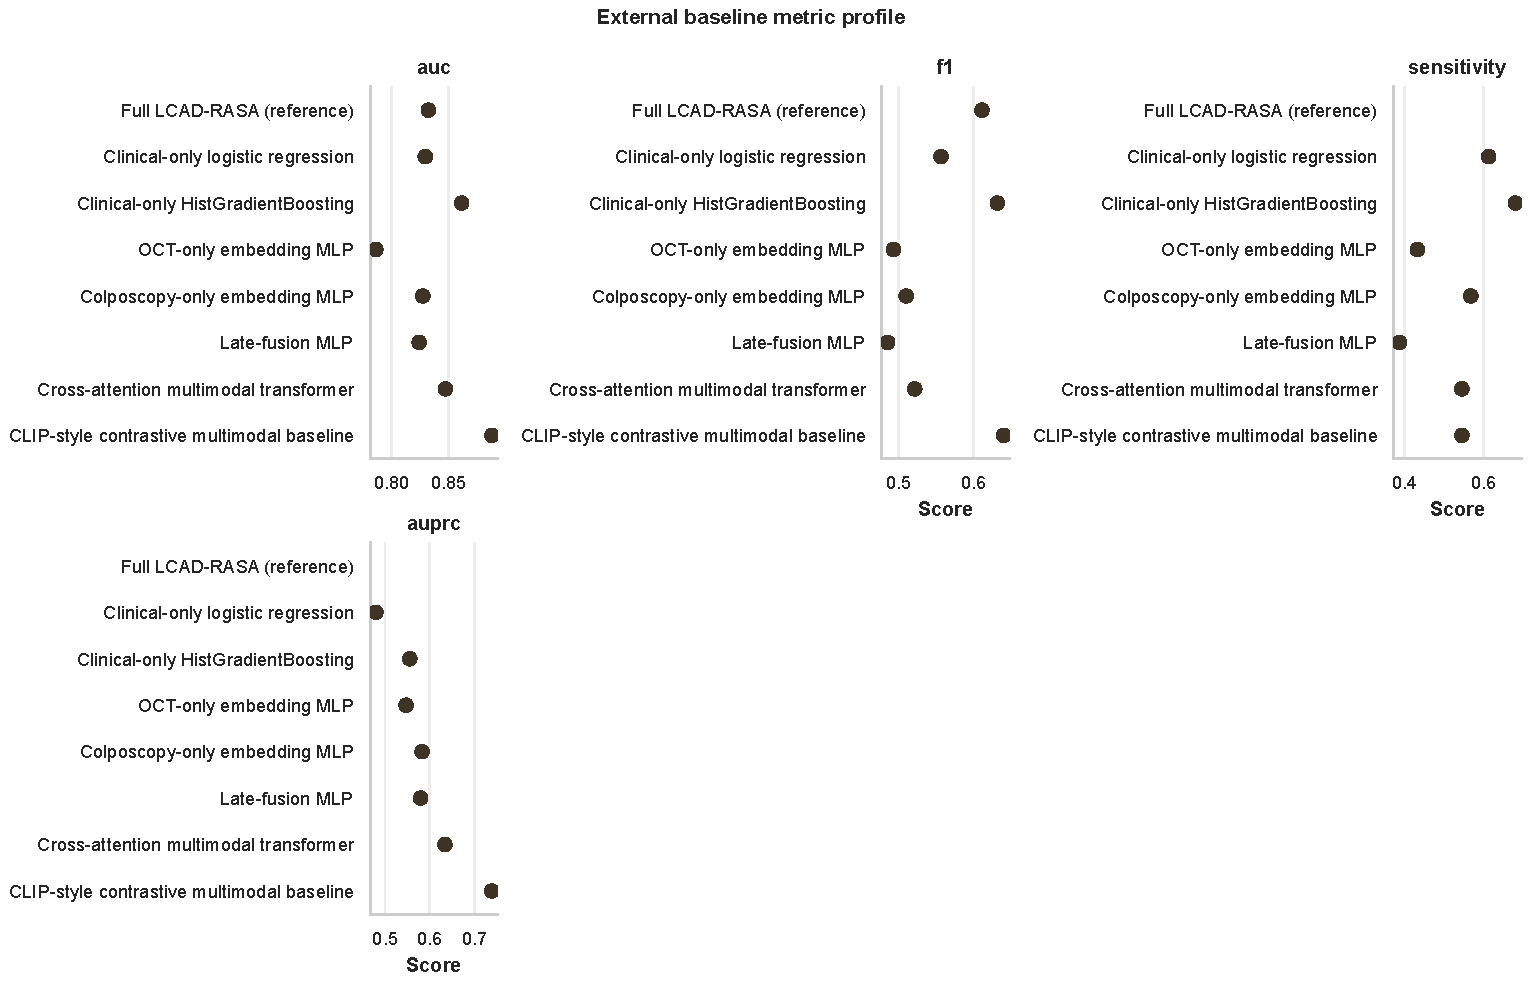
\includegraphics[width=\linewidth]{final_Fig/Figure_external_baselines_metric_dotplot.pdf}
  \caption{Supplementary metric profile of MOSAIC, the MOSAIC-RASA backbone, and external baselines under the locked held-out protocol. The dot plot compares discrimination and threshold-dependent metrics across clinical-only, image-only, late-fusion, cross-attention, contrastive, and report-aware models.}
  \label{fig:external_baselines_metrics}
\end{figure}

\begin{figure}[!htbp]
  \centering
  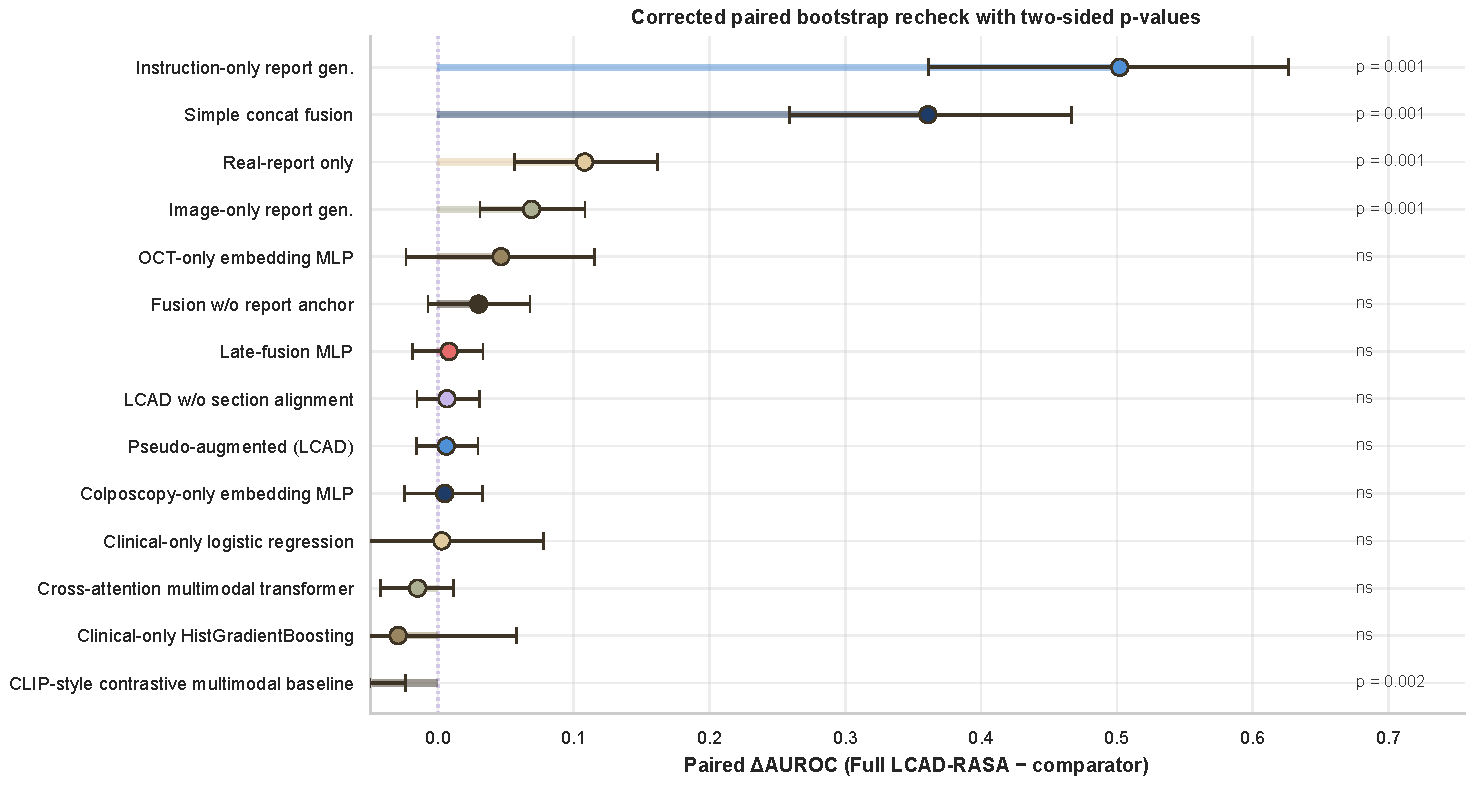
\includegraphics[width=\linewidth]{final_Fig/Figure_external_baselines_paired_delta_auc.pdf}
  \caption{Supplementary corrected paired bootstrap AUROC differences relative to the MOSAIC-RASA backbone. Positive values favour the backbone, whereas negative values favour the comparator, with intervals estimated from paired test-set resampling.}
  \label{fig:external_pairwise_recheck}
\end{figure}

\begin{figure}[!htbp]
  \centering
  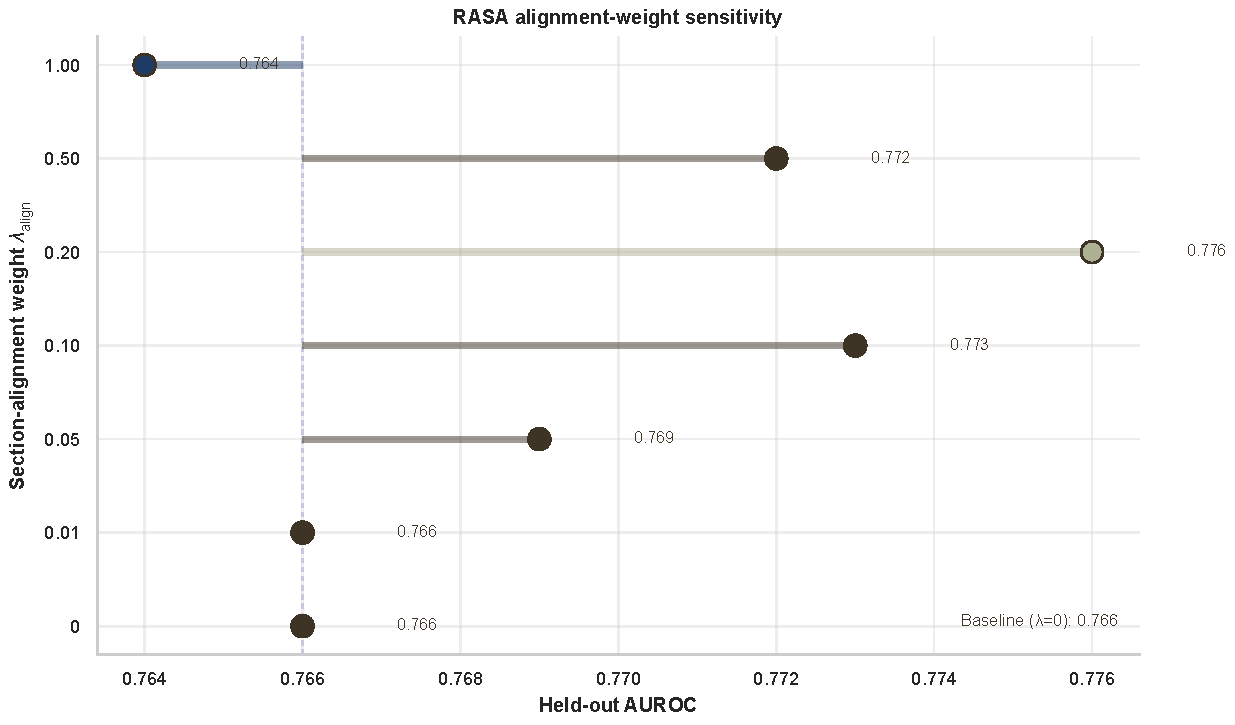
\includegraphics[width=\linewidth]{final_Fig/fig_rasa_lambda_lineplot.pdf}
  \caption{Supplementary sensitivity of model performance to the RASA alignment weight. The sweep evaluates how varying the section-alignment loss weight affects downstream discrimination and report-related metrics.}
  \label{fig:rasa_lambda}
\end{figure}

\begin{figure}[!htbp]
  \centering
  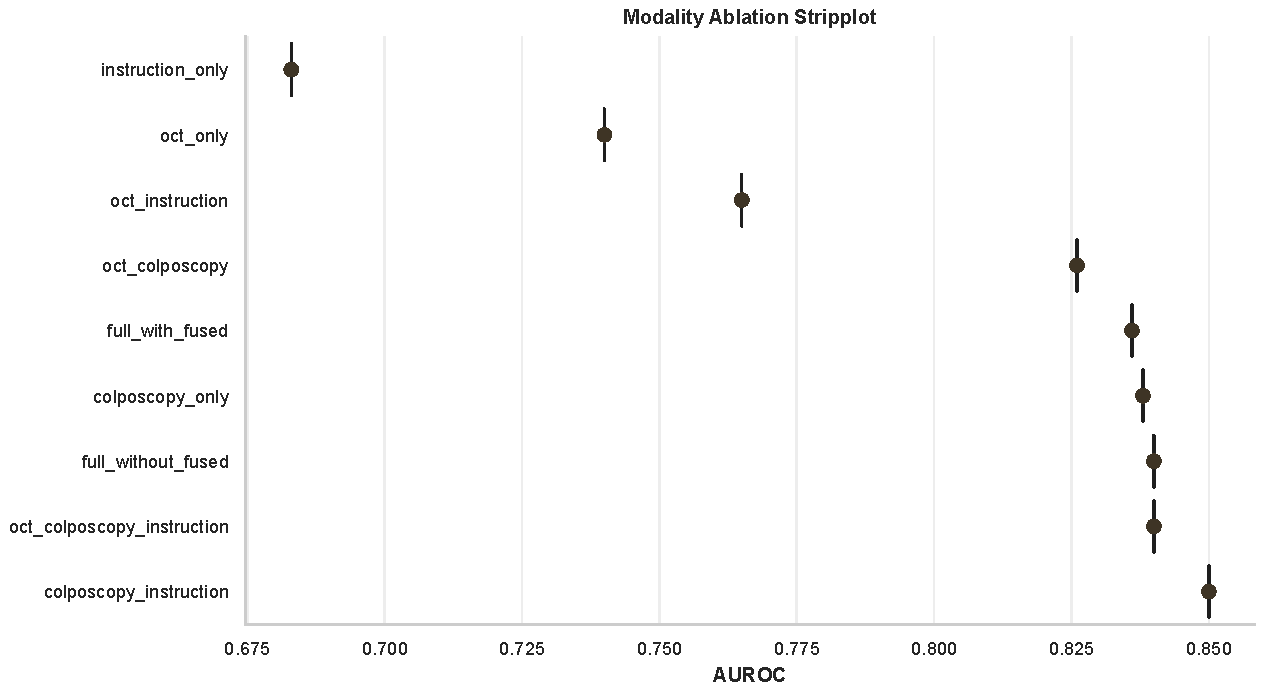
\includegraphics[width=\linewidth]{final_Fig/fig_modality_ablation_stripplot.pdf}
  \hfill
  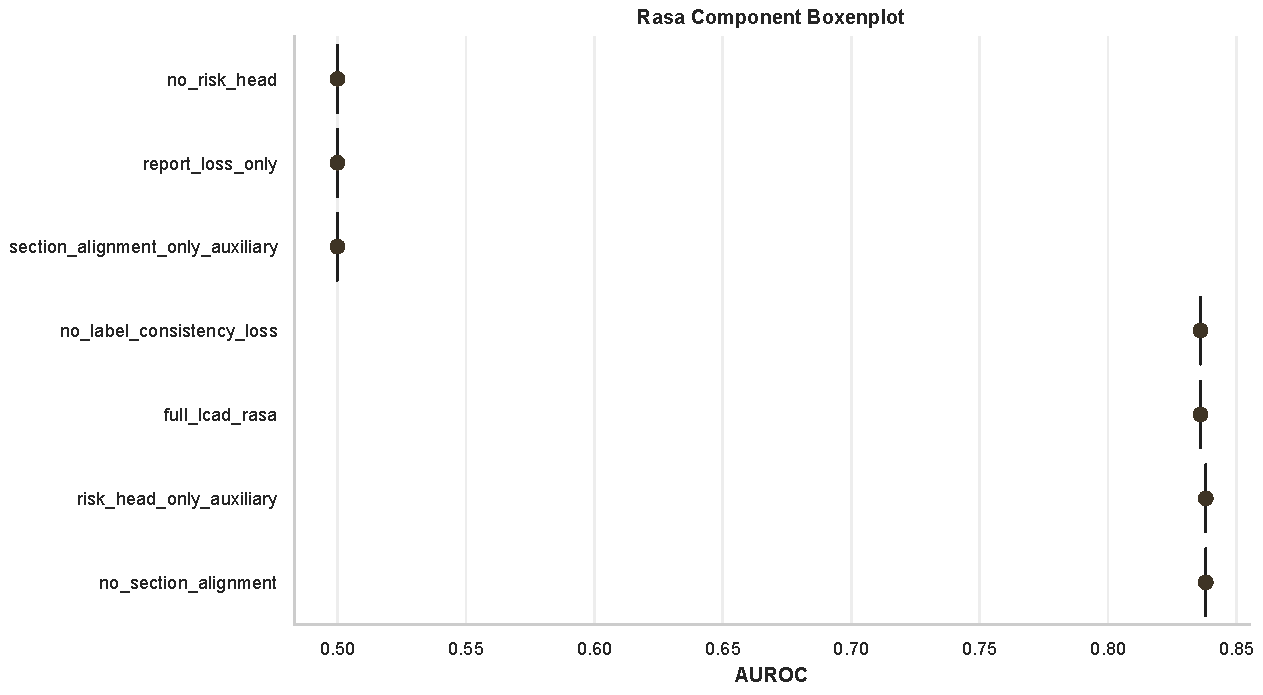
\includegraphics[width=\linewidth]{final_Fig/fig_rasa_component_boxenplot.pdf}
  \caption{Supplementary ablation analysis of modality inputs and RASA components. The panels assess the contribution of OCT, colposcopy, clinical instruction, fused visual embeddings, section alignment, risk supervision, and label-consistency terms.}
  \label{fig:rasa_component_boxenplot}
\end{figure}

\begin{figure}[!htbp]
  \centering
  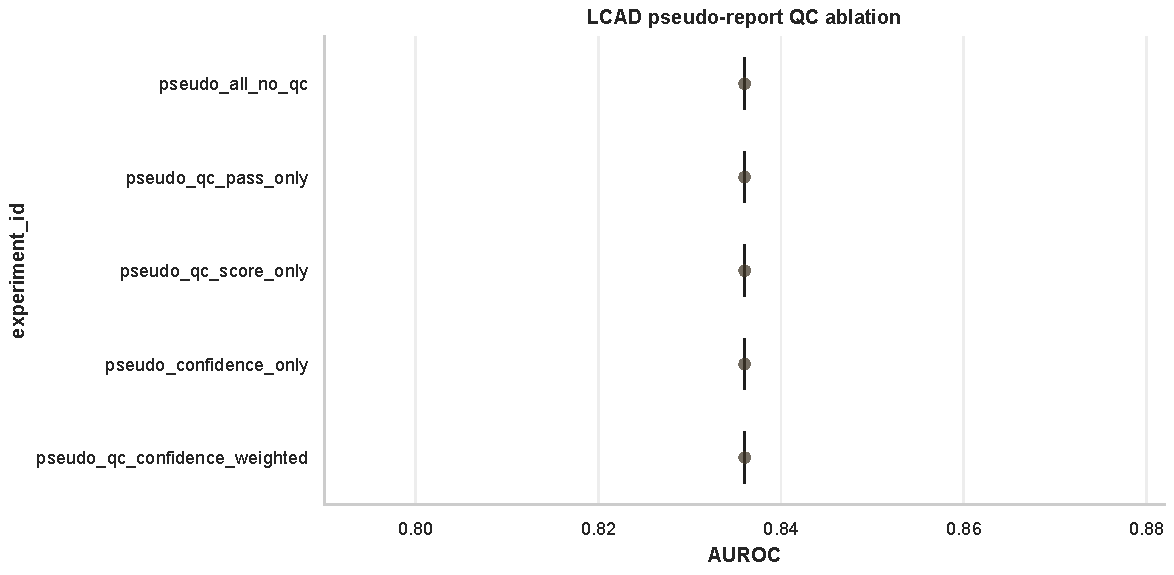
\includegraphics[width=0.82\linewidth]{final_Fig/fig_lcad_qc_ablation_barplot.pdf}
  \caption{Supplementary quality-control ablation for LCAD pseudo-report supervision. The analysis evaluates whether alternative pseudo-report filtering and weighting strategies materially alter downstream performance under the retrospective configuration; the separate failure-enriched stress test evaluates report-safety flagging rather than AUROC change.}
  \label{fig:qc_ablation}
\end{figure}

\subsection{Supplementary perturbation and modality-sensitivity figures}
These figures provide the expanded perturbation evidence behind the main perturbation matrix.

\begin{figure}[!htbp]
  \centering
  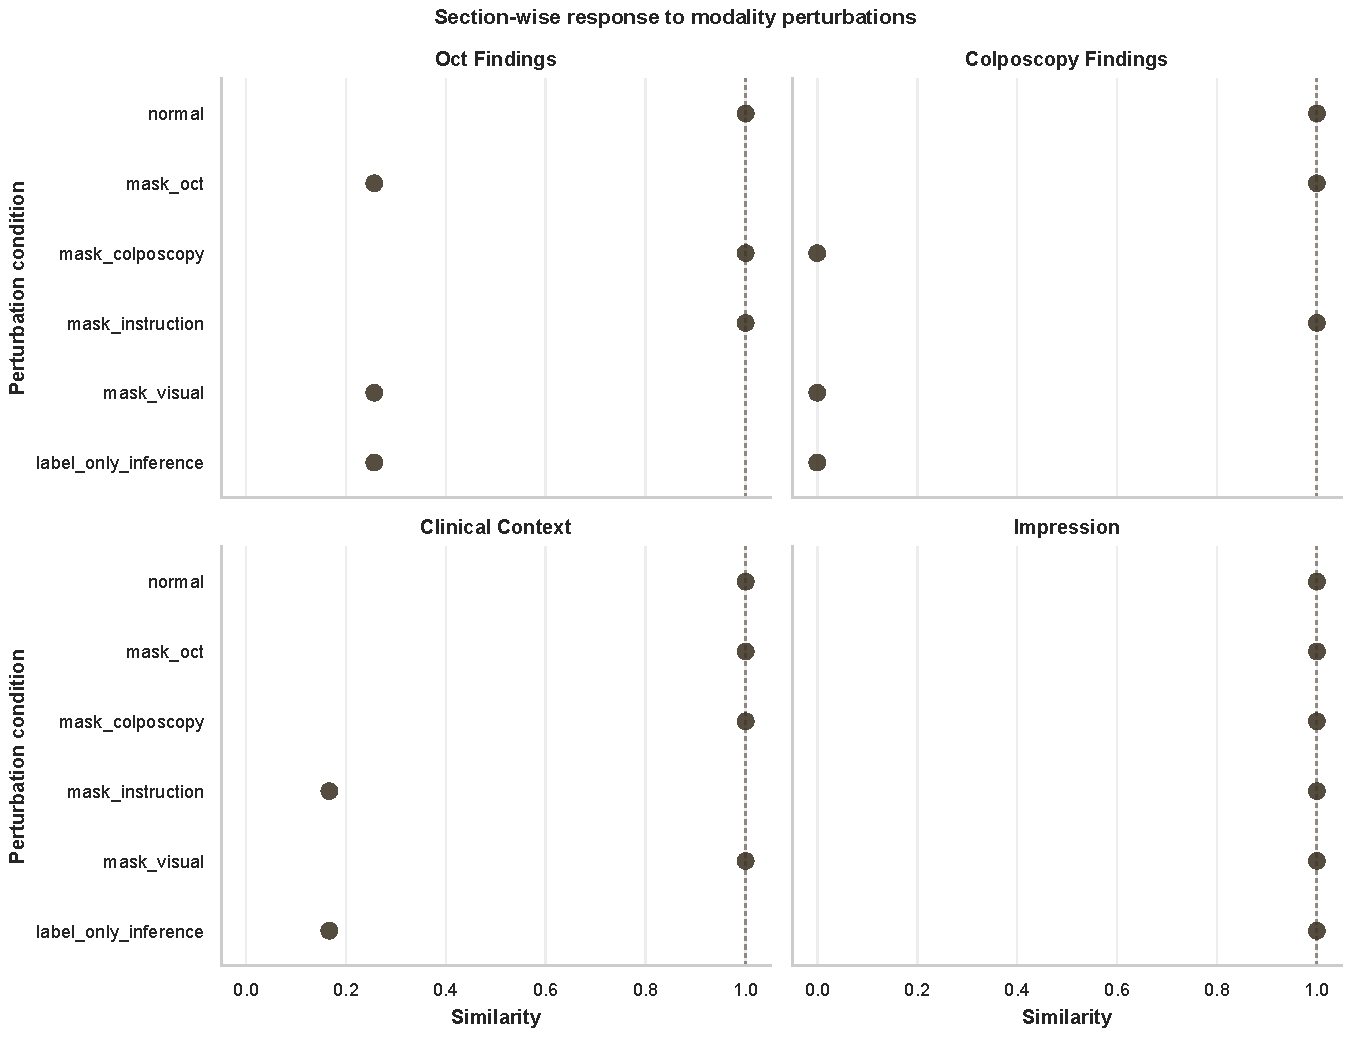
\includegraphics[width=\linewidth]{final_Fig/Figure3_modality_perturbation_lineplot.pdf}
  \caption{Supplementary section-level degradation profiles following modality-specific perturbations. The curves show whether disruption of a given input modality preferentially degrades the report section that should be grounded in that modality.}
  \label{fig:perturbation_lineplot}
\end{figure}

\begin{figure}[!htbp]
  \centering
  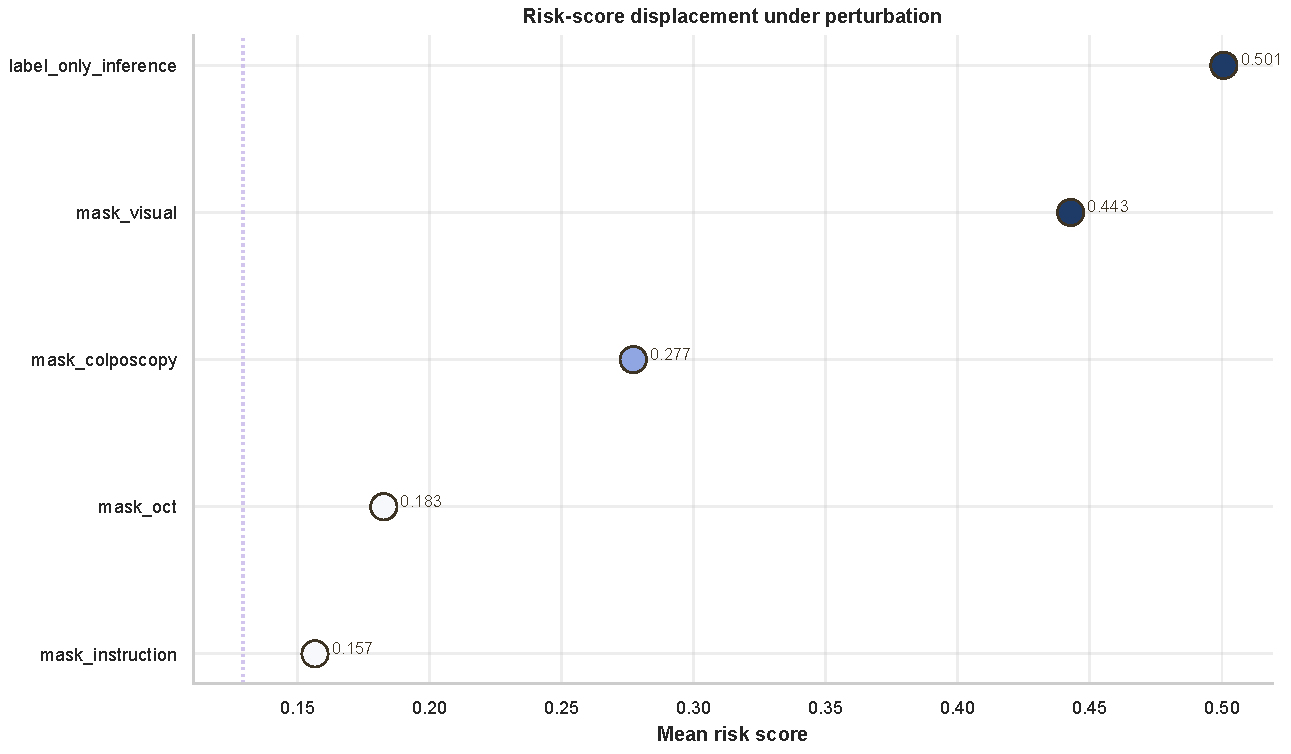
\includegraphics[width=\linewidth]{final_Fig/Figure3_risk_delta_stripplot.pdf}
  \caption{Supplementary risk-score sensitivity to report-generation perturbations. Absolute changes in predicted risk quantify the extent to which modality masking, modality shuffling, and label-only inference alter the model's diagnostic output.}
  \label{fig:risk_delta}
\end{figure}

\begin{figure}[!htbp]
  \centering
  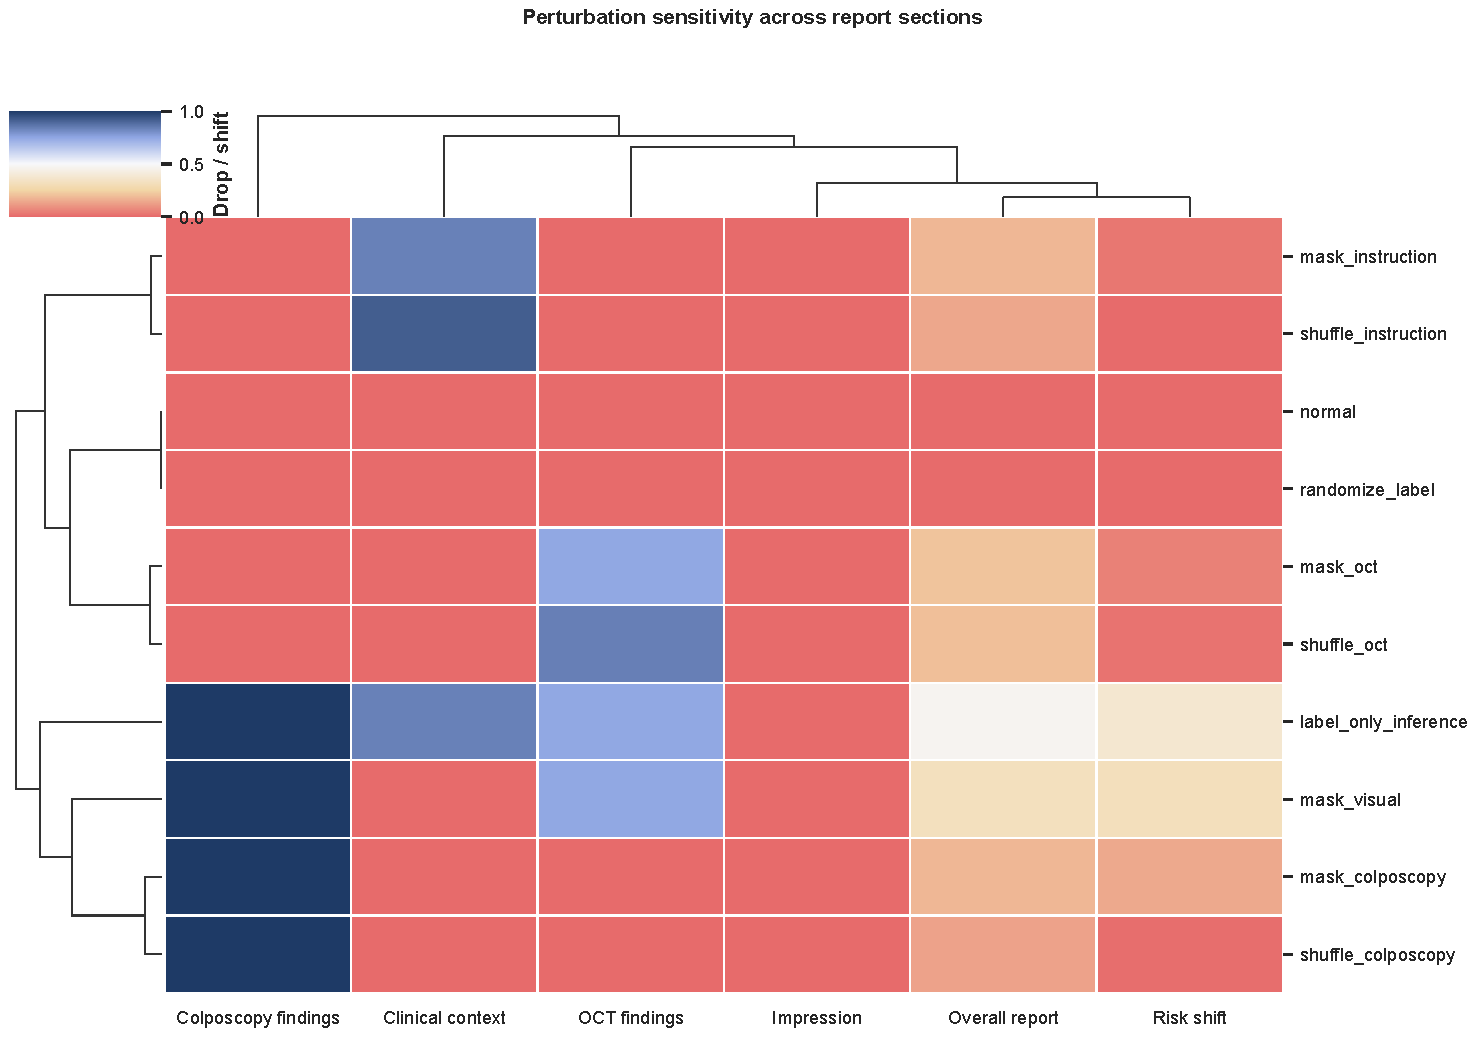
\includegraphics[width=\linewidth]{final_Fig/Figure_theme1_perturbation_sensitivity_matrix.pdf}
  \caption{Supplementary upgraded perturbation sensitivity matrix for Theme 1 cross-modal semantic alignment. The matrix consolidates section-level degradation, report-level degradation, risk shift, and specificity of the expected modality-section response.}
  \label{fig:theme1_perturbation}
\end{figure}

\subsection{Supplementary cross-centre, robustness, safety, masking, and scalability evidence}
These tables and figures complete the robustness evidence: eval-only LOCO, LOCO heatmap, multi-seed stability, report safety, masking validation, runtime and storage scale, and robustness visual summaries.

\begin{table*}[!htbp]
  \centering
  \caption{Supplementary Table S2b. Eval-only LOCO using the global checkpoint.}
  \label{tab:s2b_loco_eval_only_global_ckpt}
  \scriptsize
  \begin{threeparttable}
  \resizebox{\linewidth}{!}{%
  \begin{tabular}{llrrrr}
    \toprule
    \textbf{\makecell[l]{Held-out centre\\($n$; label consistency)}} & \textbf{Model} & \textbf{AUROC} & \textbf{F1} & \textbf{Sensitivity} & \textbf{Specificity} \\
    \midrule
    \multirow{4}{*}{\makecell[l]{Enshi\\(288; 0.741)}} 
      & Real-report-only decoder            & 0.809 & 0.500 & 0.374 & \underline{0.944} \\
      & Simple concatenation fusion         & 0.424 & 0.480 & \textbf{1.000} & 0.000 \\
      & LCAD without section alignment      & \textbf{0.863} & \textbf{0.636} & \underline{0.527} & 0.939 \\
      & MOSAIC-RASA backbone                     & \underline{0.821} & 0.122 & 0.066 & \textbf{0.995} \\
    \addlinespace[2pt]
    \multirow{4}{*}{\makecell[l]{Jingzhou\\(288; 0.587)}}
      & Real-report-only decoder            & 0.830 & 0.000 & 0.000 & \textbf{1.000} \\
      & Simple concatenation fusion         & 0.652 & 0.000 & 0.000 & \textbf{1.000} \\
      & LCAD without section alignment      & \textbf{0.877} & \textbf{0.200} & \textbf{0.111} & \textbf{1.000} \\
      & MOSAIC-RASA backbone                     & \underline{0.848} & 0.000 & 0.000 & \textbf{1.000} \\
    \addlinespace[2pt]
    \multirow{4}{*}{\makecell[l]{Xiangyang\\(288; 0.648)}}
      & Real-report-only decoder            & 0.657 & 0.071 & 0.038 & \underline{0.996} \\
      & Simple concatenation fusion         & 0.506 & 0.000 & 0.000 & \textbf{1.000} \\
      & LCAD without section alignment      & \textbf{0.864} & \underline{0.545} & 0.396 & 0.987 \\
      & MOSAIC-RASA backbone                     & \underline{0.850} & 0.203 & 0.113 & \textbf{1.000} \\
    \addlinespace[2pt]
    \multirow{4}{*}{\makecell[l]{Wuda\\(89; 0.955)}}
      & Real-report-only decoder            & 0.736 & 0.159 & 0.086 & \textbf{1.000} \\
      & Simple concatenation fusion         & 0.548 & 0.024 & 0.012 & \textbf{1.000} \\
      & LCAD without section alignment      & \textbf{0.901} & \textbf{0.970} & \textbf{1.000} & 0.375 \\
      & MOSAIC-RASA backbone                     & \underline{0.894} & \underline{0.936} & \underline{0.901} & 0.750 \\
    \addlinespace[2pt]
    \multirow{4}{*}{\makecell[l]{Shiyan\\(288; 0.566)}}
      & Real-report-only decoder            & 0.592 & 0.000 & 0.000 & 0.968 \\
      & Simple concatenation fusion         & 0.444 & 0.022 & \textbf{0.250} & 0.701 \\
      & LCAD without section alignment      & \textbf{0.747} & \textbf{0.400} & \textbf{0.250} & \textbf{1.000} \\
      & MOSAIC-RASA backbone                     & \underline{0.735} & 0.000 & 0.000 & \textbf{1.000} \\
    \bottomrule
  \end{tabular}%
  }
  \begin{tablenotes}[flushleft]
    \footnotesize
    \item Eval-only LOCO is reported separately from strict LOCO retraining and is not pooled with strict LOCO results. Repeated $n$ and label-consistency values were merged into the centre column.
  \end{tablenotes}
  \end{threeparttable}
\end{table*}

\begin{figure}[!htbp]
  \centering
  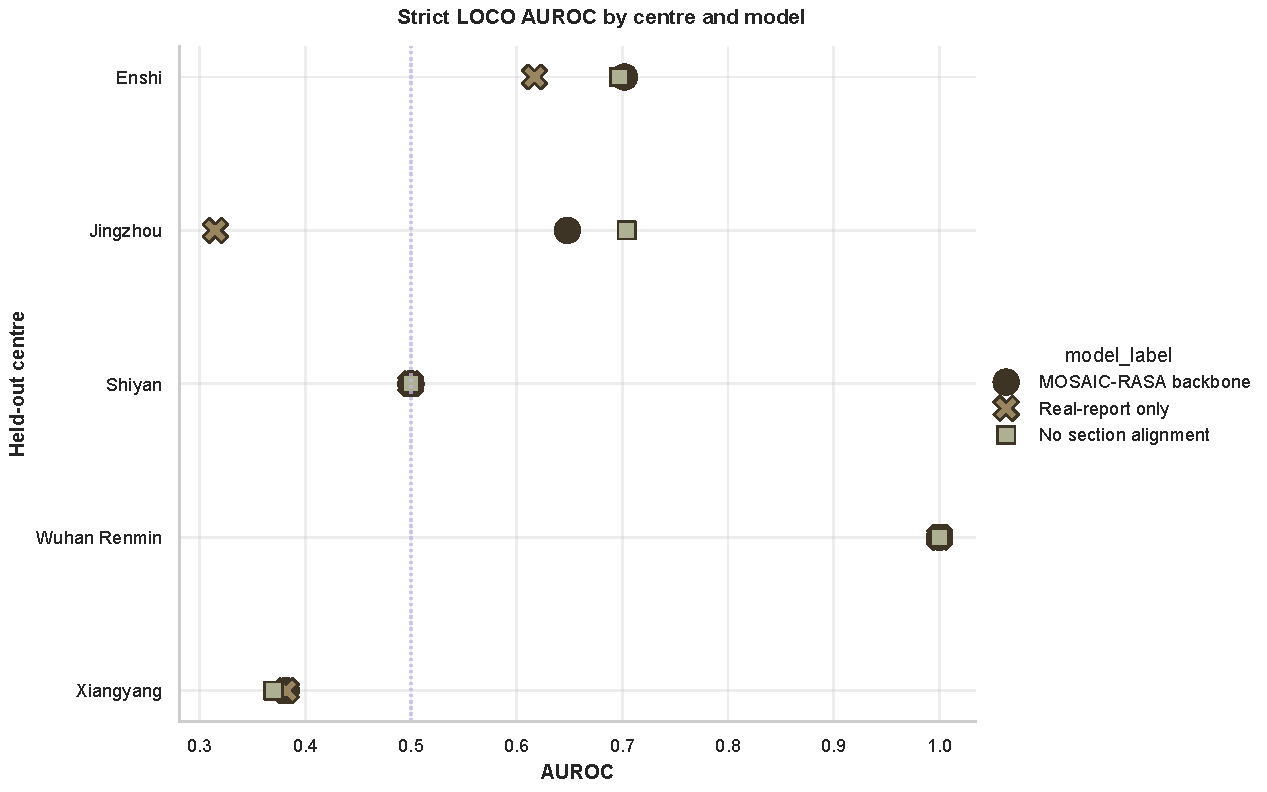
\includegraphics[width=1\linewidth]{final_Fig/fig_loco_heatmap.pdf}
  \caption{Supplementary leave-one-centre-out evaluation across participating centres. The panels summarise centre-wise AUROC patterns and strict LOCO performance, illustrating the extent of distribution shift under centre-held-out evaluation.}
  \label{fig:loco_heatmap}
\end{figure}

\begin{table*}[!htbp]
  \centering
  \caption{Supplementary Table S7. Multi-seed AUROC stability.}
  \label{tab:s7_multiseed_stability}
  \scriptsize
  \begin{threeparttable}
  \resizebox{\linewidth}{!}{%
  \begin{tabular}{lrrr}
    \toprule
    \textbf{Model} & \textbf{Mean AUROC} & \textbf{95\% interval} & \textbf{SD} \\
    \midrule
    MOSAIC-RASA backbone                    & \underline{0.776} & [0.773, 0.781] & 0.004 \\
    Report generation without section alignment & \textbf{0.780} & [0.767, 0.795] & 0.012 \\
    Real-report-only decoder                 & 0.667 & [0.656, 0.679] & 0.010 \\
    \bottomrule
  \end{tabular}%
  }
  \begin{tablenotes}[flushleft]
    \footnotesize
    \item The original metric-by-row table contained several constant rows. Across all seeds and models, mean F1 was 0.510, section completeness was 1.000, hallucination rate was 0.000, and label consistency was 0.641; the table therefore reports the variable stability metric, AUROC.
  \end{tablenotes}
  \end{threeparttable}
\end{table*}

\begin{table*}[!htbp]
  \centering
  \caption{Supplementary Table S9. Report-level safety metrics.}
  \label{tab:s9_report_safety_metrics}
  \scriptsize
  \begin{threeparttable}
  \resizebox{\linewidth}{!}{%
  \begin{tabular}{lrrrrr}
    \toprule
    \textbf{Evaluated settings} & \textbf{\makecell{Missing-modality\\hallucination}} & \textbf{\makecell{Label-report\\contradiction}} & \textbf{\makecell{Recommendation\\contradiction}} & \textbf{\makecell{Section\\incompleteness}} & \textbf{\makecell{Any\\hallucination}} \\
    \midrule
    \makecell[l]{Real-report-only decoder;\\Simple concatenation fusion;\\No section alignment;\\MOSAIC-RASA backbone;\\Pseudo reports, no QC;\\QC-confidence weighted pseudo reports}
    & 0.000 & 0.847 & 0.000 & 0.000 & 0.000 \\
    \bottomrule
  \end{tabular}%
  }
  \begin{tablenotes}[flushleft]
    \footnotesize
    \item All evaluated settings had identical values in the current legacy rule-based safety table; duplicate rows were merged. The label-report contradiction scalar is definition-sensitive and is not used as a main-text safety endpoint. The refreshed failure-enriched QC stress test is reported as the primary report-safety filtering audit.
  \end{tablenotes}
  \end{threeparttable}
\end{table*}

\begin{table*}[!htbp]
  \centering
  \caption{Supplementary Table S10. Masking validation across agent settings and centres.}
  \label{tab:s10_masking_validation}
  \scriptsize
  \begin{threeparttable}
  \resizebox{\linewidth}{!}{%
  \begin{tabular}{llrrrrr}
    \toprule
    \textbf{Setting} & \textbf{Centre} & \textbf{$n$} & \textbf{Label consistency} & \textbf{ROUGE-L} & \textbf{BLEU} & \textbf{METEOR} \\
    \midrule
    \multirow{4}{*}{Label-only agent}
      & Enshi                  & 406 & 0.659 & 0.152 & 0.081 & 0.124 \\
      & Jingzhou               & 334 & 0.513 & 0.145 & 0.076 & 0.118 \\
      & Xiangyang              & 4   & 0.500 & 0.150 & 0.080 & 0.120 \\
      & Enshi--Jingzhou pooled & 740 & 0.593 & 0.149 & 0.079 & 0.121 \\
    \addlinespace[2pt]
    \multirow{4}{*}{\makecell[l]{Modality-only agent;\\Modality-plus-label agent}}
      & Enshi                  & 406 & \textbf{0.746} & \textbf{0.251} & \textbf{0.152} & \textbf{0.203} \\
      & Jingzhou               & 334 & 0.564 & 0.238 & 0.144 & 0.195 \\
      & Xiangyang              & 4   & \underline{0.750} & 0.245 & 0.148 & 0.200 \\
      & Enshi--Jingzhou pooled & 740 & 0.664 & \underline{0.246} & \underline{0.149} & \underline{0.198} \\
    \bottomrule
  \end{tabular}%
  }
  \begin{tablenotes}[flushleft]
    \footnotesize
    \item The modality-only and modality-plus-label agents produced identical values across centres; duplicate rows were merged.
  \end{tablenotes}
  \end{threeparttable}
\end{table*}

\begin{table*}[!htbp]
  \centering
  \caption{Supplementary Table S11. Scalability and runtime summary.}
  \label{tab:s11_scalability_runtime}
  \scriptsize
  \begin{threeparttable}
  \resizebox{\linewidth}{!}{%
  \begin{tabular}{lr}
    \toprule
    \textbf{Metric} & \textbf{Value} \\
    \midrule
    \multicolumn{2}{l}{\textbf{Cohort and image scale}} \\
    Total cases & 1,897 \\
    Total centres & 5 \\
    Total images & 137,591 \\
    OCT images & 129,030 \\
    Colposcopy images & 8,561 \\
    Mean images per case & 72.531 \\
    Median images per case & 123 \\
    Maximum images per case & 144 \\
    Real-report cases & 744 \\
    Pseudo-report cases & 1,153 \\
    Missing-report rate & 0.608 \\
    \addlinespace[2pt]
    \multicolumn{2}{l}{\textbf{Storage and checkpoint size}} \\
    Embedding storage & 47.349 MB \\
    Embedding files & 5,691 \\
    Publishable checkpoint size, MOSAIC-RASA backbone / pseudo-augmented / real-report-only & 79.882 MB \\
    Publishable checkpoint size, simple fusion / fusion plus section alignment & 79.879 MB \\
    \bottomrule
  \end{tabular}%
  }
  \end{threeparttable}
\end{table*}

\begin{figure}[!htbp]
  \centering
  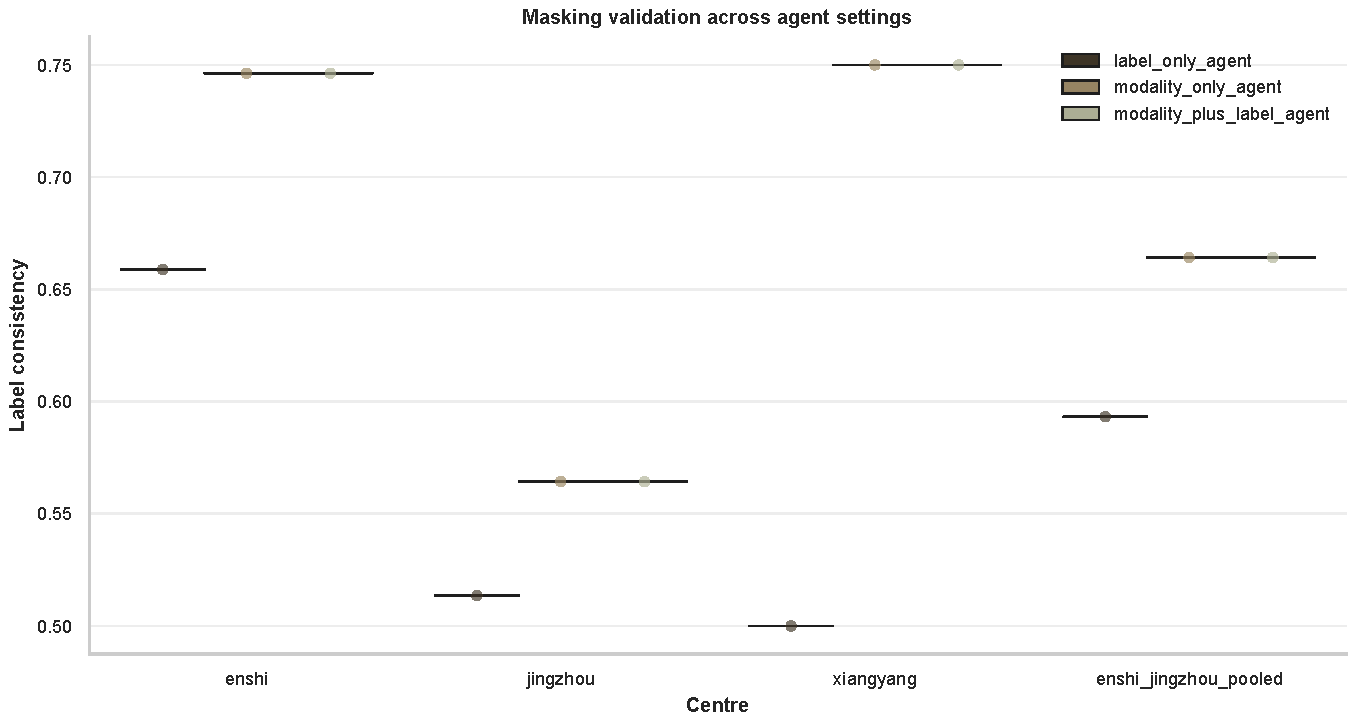
\includegraphics[width=\linewidth]{final_Fig/SupplementaryFigure_S1_masking_validation.pdf}
  \hfill
  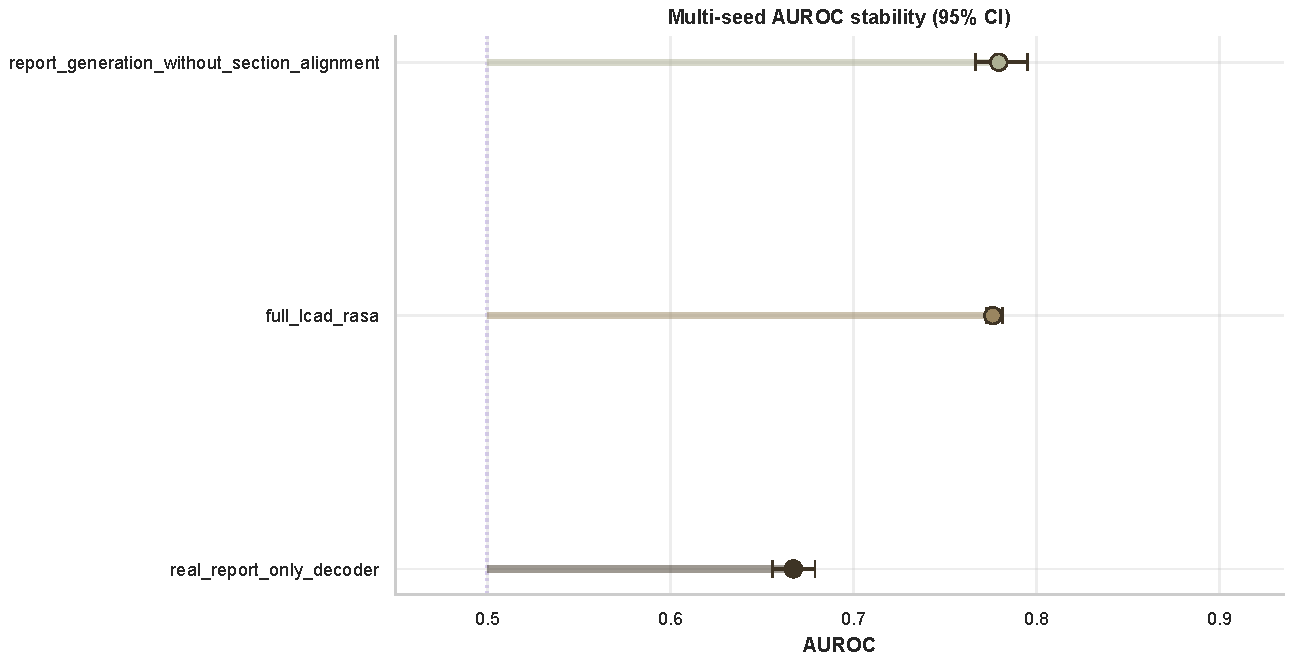
\includegraphics[width=\linewidth]{final_Fig/SupplementaryFigure_S3_multiseed.pdf}
  \caption{Supplementary robustness analyses. The panels summarise masking-validation behaviour and multi-seed stability, providing additional evidence on reproducibility and sensitivity of the retrospective pipeline.}
  \label{fig:supplementary_robustness}
\end{figure}
